% This is samplepaper.tex, a sample chapter demonstrating the
% LLNCS macro package for Springer Computer Science proceedings;
% Version 2.20 of 2017/10/04
%
\documentclass[runningheads]{llncs}
%
\usepackage{graphicx}
\usepackage{amsmath}
\usepackage{amssymb}
\usepackage{bm}
\usepackage{amsfonts}
\usepackage{subfig}
\usepackage{cleveref}
\usepackage[htt]{hyphenat}
\usepackage[newfloat]{minted}
\usepackage{caption}
\newenvironment{code}{\captionsetup{type=listing}}{}
\SetupFloatingEnvironment{listing}{name=Snippet}
\graphicspath{{./imgs/}}
\allowdisplaybreaks

\begin{document}
%
\title{Normalizing Flows}
%
%\titlerunning{Abbreviated paper title}
% If the paper title is too long for the running head, you can set
% an abbreviated paper title here
%
\author{Abdul Fatir Ansari \and
Devamanyu Hazarika\and
Remmy A. M. Zen}
%
\authorrunning{CS6202 Project Report - Normalizing Flows}
% First names are abbreviated in the running head.
% If there are more than two authors, 'et al.' is used.
%
\institute{National University of Singapore \\
\email{\{abdulfatir,devamanyu,remmy\}@u.nus.edu}}
%
\maketitle              % typeset the header of the contribution
%
%
%
%
\section{Introduction}
Improving inference, sampling, and density estimation in deep generative models (DGMs) are important research problems. Simple distributions (e.g., Gaussian) are often used as likelihood distributions in DGMs. However, the true distribution is often far from this simple distribution, which results in issues such as blurry reconstructions in the case of images. Latent variable models, such as VAEs, often set the variational posterior distribution $q(\mathbf{z}|\mathbf{x})$ to a factorial multivariate Gaussian distribution. Such a simplistic assumption hampers the model in multiple ways. For instance, this does not allow a multi-modal latent space distribution. Normalizing Flows allow transformation of samples from a simple distribution into samples from a complex distribution, whose density can be evaluated analytically, by applying a series of invertible transformations. In this report, we discuss a number of recent works that introduce techniques for improved variational inference and/or density estimation in deep generative models using normalizing flows. 
\section{Background}
\subsection{Autoencoder}
An Autoencoder (AE)~\cite{hinton2006reducing} is comprised of two neural networks: 1) The encoder network $f_\phi$ which transforms an input data-point $\mathbf{x} \in \mathbb{R}^d$ into a representation $\mathbf{z} \in \mathbb{R}^p$ where $p < d$ generally; 2) The decoder network $g_\theta$ which attempts to reconstruct $\mathbf{x}$ as $\mathbf{\hat{x}} \in \mathbb{R}^d$ from the representation $\mathbf{z}$. Training proceeds by minimizing the reconstruction error between $\mathbf{x}$ and $\mathbf{\hat{x}}$ and the training objective is given in Eq. (\ref{eq:ae})
\begin{align}
\phi,\theta = \underset{{\phi,\theta}}{\text{arg min }}\mathcal{L}(\mathbf{\hat{x}}, \mathbf{x})
\label{eq:ae}
\end{align}
where $\mathcal{L}$ is a suitable reconstruction error which can be the squared error $\|\mathbf{\hat{x}} - \mathbf{x}\|^2$ for real-valued observations or binary cross-entropy $\sum_{i=1}^d- \mathbf{x}|_i\log (\mathbf{\hat{x}}|_i) - (1 - \mathbf{x}|_i)\log (1 - \mathbf{\hat{x}}|_i)$ for binary observations.

\subsection{Variational Autoencoder}
The Variational Autoencoder (VAE)~\cite{kingma2013auto} combines an inference network $f_\phi$ (analogous to the encoder in AE) with a generative model $g_\theta$ (analogous to the decoder in AE). VAE maximizes the \textit{evidence lower bound} (ELBO) which can be derived as follows
\begin{align}
\log p(\mathbf{x}) = \log\int_{\mathbf{z}}p(\mathbf{x}, \mathbf{z})d\mathbf{z} &= \log\int_{\mathbf{z}}p(\mathbf{x}, \mathbf{z})\frac{q_\phi(\mathbf{z}|\mathbf{x})}{q_\phi(\mathbf{z}|\mathbf{x})}d\mathbf{z}\\
&\geq \mathbb{E}_{q_\phi(\mathbf{z}|\mathbf{x})}\left[\log\frac{p_\theta(\mathbf{x}| \mathbf{z})p(\mathbf{z})}{q_\phi(\mathbf{z}|\mathbf{x})}\right] = \mathcal{L}_{\mathrm{ELBO}}\label{eq:elbo}
\end{align}
where the last inequality comes from Jensen's inequality.

A data-point $\mathbf{x} \in \mathbb{R}^d$ is passed through the inference network $f_\phi$ which outputs the parameters of the variational distribution $q_\phi(\mathbf{z}|\mathbf{x})$. A point $\mathbf{z} \in \mathbb{R}^p$ is sampled from $q_\phi(\mathbf{z}|\mathbf{x})$ and is passed onto the generative model $g_\theta$ which attempts to reconstruct $\mathbf{x}$ as $\mathbf{\hat{x}} \in \mathbb{R}^d$. Once training is complete, the inference network and the generative model can be used separately. New samples from the VAE can be generated by sampling $\mathbf{z}$ from the prior $p(\mathbf{z})$ (generally set to $\mathcal{N}(\bm{0}, \mathbf{I})$) and plugging into the generative model.

Maximization of $\mathcal{L}_{\mathrm{ELBO}}$ using stochastic gradient descent (SGD) requires computation of $\nabla_\phi \mathbb{E}_{q_\phi(\mathbf{z}|\mathbf{x})}\left[\log\frac{p_\theta(\mathbf{x}| \mathbf{z})p(\mathbf{z})}{q_\phi(\mathbf{z}|\mathbf{x})}\right]$ which is done using the \textit{reparameterization trick}. Briefly, the reparameterization trick uses an invertible standardization function $\mathcal{S}_{\phi}(\mathbf{z})$ such that $\mathcal{S}_{\phi}(\mathbf{z}) = \epsilon$ where $\epsilon \sim p(\epsilon)$ and $p(\epsilon)$ is a simple distribution. For example, $\mathcal{S}_{\phi}(\mathbf{z})$ for a normally distributed random variable would be $\mathcal{S}_{\phi}(\mathbf{z}) = \frac{\mathbf{z}-\bm{\mu}}{\bm{\sigma}} = \epsilon$ with $p(\epsilon)$ being $\mathcal{N}(\bm{0}, \mathbf{I})$. Once such an invertible standardization function is available, $\nabla_\phi \mathbb{E}_{q_\phi(\mathbf{z}|\mathbf{x})}\left[f(\mathbf{z})\right]$ can be written as $\nabla_\phi \mathbb{E}_{p(\epsilon)}\left[f(\mathcal{S}_{\phi}^{-1}(\epsilon))\right]$ which can then be evaluated by using the chain rule as $ \mathbb{E}_{p(\epsilon)}\left[\nabla_{\mathbf{z}}f(\mathcal{S}_{\phi}^{-1}(\epsilon))\nabla_\phi\mathcal{S}_{\phi}^{-1}(\epsilon)\right]$. For more details please refer to Figurnov et al.~\cite{figurnov2018implicit}.

\section{Normalizing Flows}

Before defining normalizing flows, let's consider a univariate distribution with density function $p(x)$. Define a continuous, differentiable, and increasing function $f$. Define $y = f(x)$ where $x \sim p(x)$. The density function of the random variable $Y$ can then be derived analytically using the Cumulative Distribution Function (CDF) as follows.

\begin{align}
F_{Y}(y) &= P(Y \leq y)\\
&= P(f(X) \leq y)\\
&= P(X \leq f^{-1}(y)) = F_{X}( f^{-1}(y))
\end{align}

We end up with the CDF of the random variable $X$ at the point $f^{-1}(y)$. Now, $p(y) = F_{Y}'(y)$ by definition, where

\begin{align}
F_{Y}(y) = F_{X}( f^{-1}(y)) = \int_{-\infty}^{ f^{-1}(y)}p(x) dx
\label{eq:cdfy}
\end{align}

Differentiating Eq. (\ref{eq:cdfy}) with respect to $y$ (using the Fundamental Theorem of Calculus and the chain rule) we get

\begin{align}
p(y) = p(f^{-1}(y))\cdot \frac{df^{-1}}{dy}
\label{eq:incfn}
\end{align}

When $f$ is a decreasing function, we get $p(y) = -p(f^{-1}(y))\cdot \frac{df^{-1}}{dy}$.  For an invertible function in general, Eq. (\ref{eq:incfn}) can be written as 

\begin{align}
p(y) = p(f^{-1}(y))\cdot \left|\frac{df^{-1}}{dy}\right|
\label{eq:covuv}
\end{align}

Eq. (\ref{eq:covuv}) can be extended to the multivariate case where the derivative is replaced by the determinant of the Jacobian matrix

\begin{align}
p(\mathbf{y}) = p(f^{-1}(\mathbf{y}))\cdot \left|\det\frac{\partial f^{-1}}{\partial\mathbf{y}}\right| = p(f^{-1}(\mathbf{y}))\cdot \left|\det\frac{\partial f}{\partial f^{-1}(\mathbf{y})}\right|^{-1}
\label{eq:covmv}
\end{align}

In the above equation, the second equality comes from the inverse function theorem. Successive applications of such smooth, invertible transformation on a random variable with known density is called a \textit{normalizing flow}.

 Computation of the probability density of the transformed random variable requires the computation of the determinant of the Jacobian matrix which is computationally expensive as it scales with $O(d^3)$ where $d$ is the dimensionality of the random variable. Developing transformations with cheap determinant computation has been the primary focus of many recent works.
\section{Applications}
Literature on normalizing flows can be broadly classified into two parts: ones using normalizing flows for improved variational inference and ones using normalizing flows for density estimation.
\subsection{Variational Inference}
Variational methods perform inference by approximating the true posterior $p(\mathbf{z}|\mathbf{x})$ using a simpler variational family $q_{\phi}(\mathbf{z}|\mathbf{x})$. Recent works have focused on improving the variational posterior used in the VAE which is generally set to a multivariate normal distribution with diagonal covariance matrix $\mathcal{N}(\bm{\mu}, \sigma^2\mathbf{I})$. It is clear that such a simplistic, unimodal choice for the posterior can be arbitrarily far away from the true posterior which can be a complex multi-modal distribution. 

Recent works seek to convert samples from a simple variational posterior (such as the multivariate normal distribution) into a richer distribution by applying a series of smooth, invertible transformations or a flow. Let $\mathbf{z}_0$ be a sample from a simple distribution $q_0(\mathbf{z}_0)$ and $\mathbf{z}_K$ be a sample obtained by applying a flow of length $K$ on $\mathbf{z}_0$, i.e., $\mathbf{z}_K = f_K \circ f_{K-1} \circ \dots \circ f_1 (\mathbf{z}_0)$. Using Eq. (\ref{eq:covmv}), the density function $q_K(\mathbf{z}_K)$ is given by

\begin{align}
q_K(\mathbf{z}_K) = q_0(\mathbf{z}_0)\prod_{k=1}^K\left|\det \frac{\partial f_k}{\partial \mathbf{z}_{k-1}}\right|^{-1}\label{eq:qzk}
\end{align}

The variational lower bound in VAEs (Eq. \ref{eq:elbo}) can now be modified by setting $q(\mathbf{z}|\mathbf{x}) = q_K(\mathbf{z}_K|\mathbf{x})$
\begin{align}
\mathcal{L} &= \mathbb{E}_{q(\mathbf{z}_K|\mathbf{x})}\left[\log p_\theta(\mathbf{x}, \mathbf{z}_K) - \log q(\mathbf{z}_K|\mathbf{x})\right]\\
&= \mathbb{E}_{q(\mathbf{z}_0|\mathbf{x})}\left[\log p_\theta(\mathbf{x}, \mathbf{z}_K) - \log q(\mathbf{z}_K|\mathbf{x})\right]\label{eq:lotus}
\end{align}
where $q(\mathbf{z}_0|\mathbf{x})$ is the simple initial density. Plugging in Eq. (\ref{eq:qzk}) into Eq. (\ref{eq:lotus}), we get a modified bound for flow-based VAEs
\begin{align}
\mathcal{L} &= \mathbb{E}_{q_0(\mathbf{z_0}|\mathbf{x})}\left[\log p(\mathbf{x},\mathbf{z}_K) - \log q_0(\mathbf{z}_0|\mathbf{x}) + \sum_{k=1}^K\log\left|\det \frac{\partial f_k}{\partial \mathbf{z}_{k-1}}\right| \right]
\end{align}
\subsubsection{Planar and Radial Flow} 
Planar and Radial Flows \cite{rezende2015variational} are one of the earliest flows proposed in the context of variational inference. Planar flows apply transformations perpendicular to a plane while radial flows apply them around a point. 

Planar flows use functions of the form
\begin{align}
f(\mathbf{z}) = \mathbf{z} + \mathbf{u}h(\mathbf{w}^\top\mathbf{z} + b)
\label{eq:planarfn}
\end{align}

where $\mathbf{u},\mathbf{w}\in \mathbb{R}^d$, $b \in \mathbb{R}$, and $h$ is an element-wise non-linearity such as $\tanh$.

The Jacobian determinant is then given by
\begin{align}
\det\frac{\partial f(\mathbf{z})}{\partial \mathbf{z}} =(1 + h'(\mathbf{w}^\top\mathbf{z} + b)\mathbf{w}^\top\mathbf{u})
\end{align}
which can be computed in $O(d)$ time.

Radial flows use functions of the form
\begin{align}
f(\mathbf{z}) = \mathbf{z} + \beta h(\alpha,r)(\mathbf{z}-\mathbf{z}_0)
\label{eq:radialfn}
\end{align}

where $\alpha \in \mathbb{R}^+$, $\beta \in \mathbb{R}$, $h(\alpha,r) = (\alpha + r)^{-1}$ and $r = \vert\vert\mathbf{z} - \mathbf{z}_0\vert\vert$.

The Jacobian determinant is then given by
\begin{align}
\det\frac{\partial f(\mathbf{z})}{\partial \mathbf{z}} = \left(1 + \beta h(\alpha,r) + \beta h'(\alpha,r)r\right)(1+\beta h(\alpha,r))^{d-1}
\end{align}

For a detailed derivation of Jacobians of Planar and Radial flows please refer the appendix. Fig. \ref{fig:planarradial} shows how planar and radial flows change a standard normal density.

\begin{figure}
	\centering
	\subfloat[Initial Density]{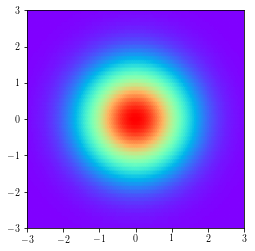
\includegraphics[width=0.24\textwidth]{planar-q0}}
	\subfloat[Planar Flow]{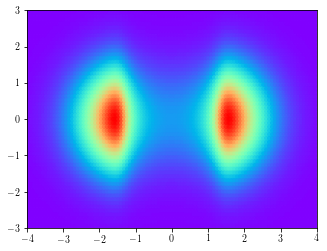
\includegraphics[width=0.31\textwidth]{planar-q1}}
	\subfloat[Radial Flow]{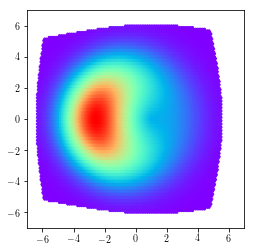
\includegraphics[width=0.24\textwidth]{radial-q1}}
	\caption{Change in standard normal density on application of length 1 planar and radial flows.}
	\label{fig:planarradial}
\end{figure}

\subsubsection{Inverse Autoregressive Flow} Planar and radial flows provide a simple invertible transformation shown to be effective in a low-dimensional latent spaces (up to hundred dimensions). The transformation in planar flows (Eq. \ref{eq:planarfn}) can be seen as a Multilayer Perceptron (MLP) with a single-unit bottleneck hidden layer with a skip connection. Since a single-unit hidden layer isn't very expressive, a long chain of transformations is needed to model a high-dimensional distribution. 

Autoregressive flows~\cite{germain2015made} is a normalizing flow that scales to high-dimensional latent space by exploiting the ordering f the variables. In autoregressive flow, given a sequence of variable $\mathbf{y} = {y_i}_{i=0}^D$, each variable is only dependent only on variables from the previous index. The distribution is then given by
\begin{align}
p(\mathbf{y}) = \prod_{i=0}^{D} p(x_i | x_0,\dots,x_{i-1})
\end{align} 	 

Kingma et. al.~\cite{kingma2016improved} proposed a Gaussian version of an autoregressive flow on a noise vector $\mathbf{\epsilon} \sim \mathcal{N}(0,\mathbf{I})$ given as follow:
\begin{align}
y_0 &= \mu_0 + \sigma_0 \epsilon_0\label{eq:iaffn1}\\
y_i &= \mu_i(\mathbf{y}_{0:i-1}) + \sigma(\mathbf{y}_{0:i-1}) \epsilon_i\label{eq:iaffn2}
\end{align} 

This flow is invertible and the noise $\epsilon$ is given by:
\begin{align}
\epsilon_i &= \frac{y_i - \mu_i(\mathbf{y}_{0:i-1})}{\sigma(\mathbf{y}_{0:i-1})}
\label{eq:iaf}
\end{align} 

Note that, $epsilon$ is independent to each other so the calculation of Equation~\ref{eq:iaf} can be vectorized as follow:
\begin{align}
\bm{\epsilon} &= \frac{\mathbf{y} - \bm{\mu}(\mathbf{y})}{\bm{\sigma}(\mathbf{y})}
\end{align} 
This enables an efficient computation with GPU. 

Due to the autoregressive structure, the transformation has a lower triangular Jacobian where diagonal is $\sigma_i$. For calculation of normalizing flows, we are interested in log-determinant of the Jacobian which is just a product of the diagonal given as:
\begin{align}
\log \det \left| \frac{d\bm{\epsilon}}{d\mathbf{y}} \right| = \sum_{i=0}^{D} - \log \sigma_i(\mathbf{y})
\end{align}

To apply Inverse Autoregressive Flows (IAF) for variational inference in VAE, we add IAF transforms after the latent variables $\mathbf{z}$ and modify the likelihood to account for IAF transforms. Figure~\ref{fig:iaf} shows the process of applying IAF to Variational Autoencoder. 

\begin{figure}[htb]
	\centering
	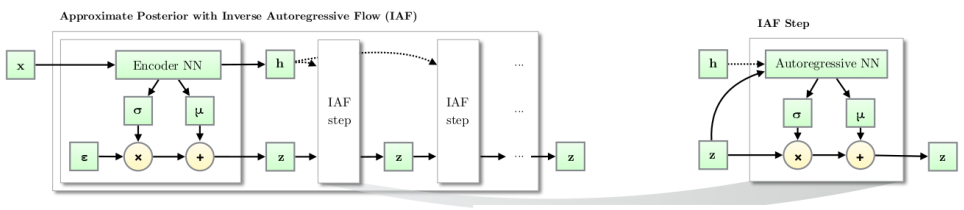
\includegraphics[width=\textwidth]{imgs/iaf}
	\caption{The process of Inverse Autoregressive Flows in Variational Autoencoder~\cite{kingma2016improved}.}
	\label{fig:iaf}
\end{figure}

The flow consists of a chain of $T$ following transformations:
\begin{align}
\mathbf{z}_t = \bm{\mu}_t + \bm{\sigma}_t\mathbf{z}_{t-1}
\end{align}

Kingma et.al.~\cite{kingma2016improved} proposed a more stable update based on LSTM-type update. LSTM is a type of recurrent neural network that applies autoregressive technique to the neural network.  The update is given as follows:
\begin{align}
\mathbf{s}_t = 1 / \sigma_t\:\text{and}\:\mathbf{m}_t = -\mu_t / \sigma_t\:\text{and}\:\sigma_t = \frac{1}{1 + e^{-\mathbf{s}_t}}\:\text{and}\:\mathbf{z}_t = \sigma_t\mathbf{z}_{t-1} + (1 - \sigma_t)\mathbf{m}_{t} 
\end{align}

where $\bm{\mu}$ and $\bm{\sigma}$ learnt from an Autoregressive neural network given in~\cite{germain2015made} receiving input $\mathbf{z}$ and $\mathbf{h}$ from the VAE. 

\subsubsection{Sylvester Normalizing Flow} As explained earlier, planar flows suffer from the single-unit bottleneck problem. Sylvester Normalizing Flows (SNF)~\cite{van2018sylvester} attempt to solve this problem by modifying the transformation function which then behaves as an MLP with $M$ units instead of 1. SNF uses a transformation function of the following form 
\begin{align}
f(\mathbf{z}) = \mathbf{z} + \mathbf{A}h(\mathbf{B}\mathbf{z} + \mathbf{b})
\label{eq:sylfn}
\end{align}
where $\mathbf{A} \in \mathbb{R}^{d\times m},\mathbf{B} \in \mathbb{R}^{m \times d}$, $b \in \mathbb{R}^{m}$ with $m \leq d$, and $h$ is an element-wise non-linearity such as $\tanh$. Using Sylvester's determinant identity, we can convert the computation of the determinant of a $d \times d$ matrix into the computation of the determinant of an $m \times m$ matrix. 
\begin{align}
\det(\mathbf{I}_d + \mathbf{A}\mathbf{B}) = \det(\mathbf{I}_m + \mathbf{B}\mathbf{A})
\end{align}
Matrices $\mathbf{A}\text{ and }\mathbf{B}$ are further parameterized as $\mathbf{A} = \mathbf{Q}\mathbf{R}$ and $\mathbf{B} = \mathbf{\tilde{R}}\mathbf{Q}^\top$ where $\mathbf{R}\text{ and }\mathbf{\tilde{R}}$ are $m\times m$ upper-triangular matrices and $\mathbf{Q}$ is $d \times m $ matrix with orthonormal column vectors. The determinant of the Jacobian can then be written as
\begin{align}
\frac{\partial f(\mathbf{z})}{\partial \mathbf{z}} = \det \left(\mathbf{I}_m + \mathrm{diag}\left(h'(\mathbf{\tilde{R}}\mathbf{Q}^\top\mathbf{z} + \mathbf{b})\right)\mathbf{\tilde{R}}\mathbf{R}\right)
\end{align}
which can be computed in $O(m)$ time. Please refer to the original paper~\cite{van2018sylvester} for details.

\subsection{Density Estimation}
Density Estimation techniques take a different approach from Variational Inference (VI) methods to model the complex data distribution. Unlike VI, these methods aim for exact inference, sampling and log-likelihood evaluation. The primary goal in this regime is to find a bijective function $h=f(x)\;,x \in \mathcal{X}$ to map complex data-distribution $p_X(x)$ to density $p_H(f(x))$. Given that $p_H()$ has a simpler density whose likelihood function is analytically known, the overall log-likelihood of the data can be easily calculated. The complex log-likelihood of the data can now be calculated using the change of variables as follows:
\begin{align}
\log p_X(x)  = \log p_H(f(x)) +
\log\left| \det\frac{\partial f(x)}{\partial x} \right| \label{eq:log-likelihood}
\end{align}

\subsubsection{Non-linear Independent Components Estimation} \label{sec:nice}

Non-linear Independent Components Estimation (NICE) \cite{dinh2014nice} is one of the early works adopting normalizing flows in density estimation. This work focuses on transformations $h=f(x)$ that maps the data into a factorized distribution, i.e., the components of $h_d$ are independent. Consequently, the log-likelihood in \cref{eq:log-likelihood} can be written as:
\begin{align}
\log(p_X(x)) = \left[\sum_{d=1}^{D}  \log p_{H_d}(f_d(x))\right] +
\log\left| \det\frac{\partial f(x)}{\partial x} \right|
\end{align}
where $f(x) = (f_{d}(x))_{d \leq D}$.

This work targets invertible functions whose Jacobians have triangular structure so that calculating the determinant is tractable. In particular, it proposes the family of \textit{coupling layers} that we define below.

\paragraph{Coupling layer:} The coupling layer serves a building block of the transformation proposed in this work. The general coupling layer comprises of two partitions $I_{1}, I_{2}$ of the input dimensions  $\left[ 1, D \right]$, such that $d = \lvert I_{1} \rvert$. The transformation is then defined as:
\begin{align}
y_{I_{1}} &= x_{I_{1}} \\
y_{I_{2}} &= g(x_{I_{2}} ; m(x_{I_{1}}))
\end{align}
where
$g: \mathbb{R}^{D-d} \times m(\mathbb{R}^{d}) \rightarrow \mathbb{R}^{D-d}$ is an invertible function. Considering 
$I_{1} = \left[ 1, d \right]$ and $I_{2} = \left[ d, D \right]$,
the Jacobian of this function is:
\begin{align*}
\frac{\partial y}{\partial x} =
\begin{bmatrix}
I_{d} & 0 \\
\frac{\partial y_{I_{2}}}{\partial x_{I_{1}}} & \frac{\partial y_{I_{2}}}{\partial x_{I_{2}}} 
\end{bmatrix}
\end{align*}
Where $I_{d}$ is the identity matrix of size $d$. That means that
$\det \frac{\partial y}{\partial x} = \det \frac{\partial y_{I_{2}}}{\partial x_{I_{2}}}$ which evaluates to $1$. 
The inverse of this transformation can be expressed as $x_{I_{1}} = y_{I_{1}}$ and $x_{I_{2}} = g^{-1}(y_{I_{2}} ; m(y_{I_{1}}))$:

It is important to notice that the inverse of coupling function $m(.)$ is not required, thus allowing it to be modeled as complex non-linear functions. NICE adopts an \textit{additive coupling law} which defines the function $g(.)$ as $g(a,b)\,=\,a+b$. Also, reLU is chosen as the coupling function $m(.)$.

A single coupling layer leaves part of the input unchanged. This is problematic, since modification of every dimension is desired. To achieve this, roles of partitions are interachanged in arjacent layers to ensure proper mixing. 
 
\subsubsection{Real-valued Non-Volume Preserving} \label{sec:realnvp}
This subsequent work (RealNVP) \cite{dinh2016density} is an extension to the previous work (NICE) to enable multi-scalable architecture. The model uses \textit{affine coupling law} as its primary constituent. This is defined as:
\begin{align}
y_{1:d} &= x_{1:d}\\
y_{d+1:D} &= x_{d+1:D} \odot \exp\big(s(x_{1:d})\big) + t(x_{1:d})
\end{align}
where $I_1 = [1,d]$ and $I_2 = [(d+1),D]$. Also, $\exp(s(.))$ represents the \textit{scale} and $t(.)$ represents the \textit{shift} operation respectively. The Jacobian of this transformation is also a triangular matrix (derivation has been provided in appendix).

Apart from the affine transformation, the model also proposes partitioning schemes across channels of input images and checkerboard pattern-based partitioning for exploiting pixel correlations. Further, to enable deep networks, the work proposes using techiniques such as Gaussianization and invertible \textit{batch-normalization}. It achieves to get competitive scores against state-of-the variants, with some advantages that are discussed in the appendix.

\subsubsection{Masked Autoregressive Flow} The section on Inverse Autoregressive Flow (IAF) has already described how Autoregressive models such as MADE~\cite{germain2015made} can be used as normalizing flows. Masked Autoregressive Flow (MAF)~\cite{papamakarios2017masked} uses the transformation function in Eq. (\ref{eq:iaffn2}) contrary to IAF which uses the inverse function. Since the inverse function can be parallelized, MAF is suitable for computation of the density $p(\mathbf{x})$ of an externally provided data point $\mathbf{x}$. Sampling a new point from MAF requires $D$ sequential passes which cannot be parallelized and hence sampling is slow. However, in the case of IAF, as the inverse function is used, sampling is fast but density estimation is slow and requires $D$ sequential passes.

\section{Normalizing Flows in Probabilistic Programming Languages}
Normalizing flows have been implemented in two recent deep probabilistic programming languages Pyro (based on Pytorch) and Tensorflow Probability (TFP, based on Tensorflow). They provide a construct called the \texttt{Bijector} for the implementation of an invertible transformation required for construction of a normalizing flow. New transformation functions can be defined by extending the \texttt{Bijector} class. TFP also provides a construct called the \texttt{TransformedDistribution} which takes in a base distribution (which is generally a simple distribution) and a \texttt{Bijector}. A \texttt{TransformedDistribution} represents the distribution obtained after applying the \texttt{Bijector} on the base distribution. A number of functions commonly used in deep learning (e.g., Affine, Sigmoid, RealNVP) have been implemented as \texttt{Bijector}s in TFP. Another bijector called \texttt{Chain} is provided in TFP that converts a list of bijectors into a single bijector which represents a flow. The complete documentation of normalizing flows in TFP is given in~\cite{dillon2017tensorflow}.

Defining a custom transformation requires extending the \texttt{Bijector} class and implementing three functions: 1) \texttt{\_forward} -- receives samples $x$ from the base distribution as an input, evaluates the function $y = f(x)$, and returns the variable $y$. 2) \texttt{\_inverse} -- receives $y$ as the input and outputs $x$ corresponding to the inverse of the function, i.e., $x = f^{-1}(y)$. 3) \texttt{\_inverse\_log\_det\_jacobian} -- receives $y$ as the input and computes the inverse log-determinant of the Jacobian, i.e., $\log \det \left|\frac{\partial f^{-1}}{\partial y}\right|$. 

Let's define the three functions for an example function, the Parametrized ReLU (PReLU) function.
\begin{align}
y = f(x) &= \begin{cases}
x\quad&\text{if } x \geq 0\\
\alpha x\quad&\text{otherwise, where }\alpha\in [0, 1]
\end{cases}\\
x = f^{-1}(y) &= \begin{cases}
y\quad&\text{if } y \geq 0\\
\alpha^{-1} y\quad&\text{otherwise}
\end{cases}\\
\frac{\partial f^{-1}}{\partial y}\Bigg|_{ii} &= 
\begin{cases}
1\quad&\text{if } y_i \geq 0\\
\frac{1}{\alpha}\quad&\text{otherwise}\\
\end{cases}
\end{align}
An example bijector implementation for the PReLU function is given in the appendix.

\section{Recent Advances}
In this section, we discuss several recent works that used normalizing flows. We only explain the higher-level concept of each work. Interested readers should refer to the original paper given in the reference.
\subsection{Pixel Recurrent Neural Network}
Pixel Recurrent Neural Network (PixelRNN)~\cite{oord2016pixel} is an auto-regressive image generative model where the joint distribution over the image pixel is factorized into a product of conditional distribution. This means that the probability of pixel at position $i$ is given as: $p(x_i | x_1, \dots, x_{i-1})$ where $x_1, \dots, x_{i-1}$ is the previously generated pixels. This is a strong and counter-intuitive assumption for an image generation where pixel mostly conditioned on their neighbors. However, PixelRNN is proven to  work well for image completion and generation task. In image completion, the occluded pixel is generated by conditioned upon the non-occluded pixels.

Oord et. al.~\cite{oord2016pixel} proposed three methods model an auto-regressive image generation.  First, Row LSTM 1D convolution is used to generate image row by row from top to bottom. However, Row LSTM cannot capture the whole previously generated pixels since there is a coarse-graining in the convolution method. Second, Bidirectional LSTM is used to capture all the generated pixels as the context. Every pixel is conditioned upon their neighboring pixels except the one that has not been generated. However, LSTM training is known to be expensive so the authors proposed another model based on CNN. Third, Pixel CNN used a masked convolution by setting the filter of the pixels that has not been generated as zero.

% Each method is visualize in Figure~\ref{fig:pixelrnn}. 
%\begin{figure}[htb]
%	\centering
%	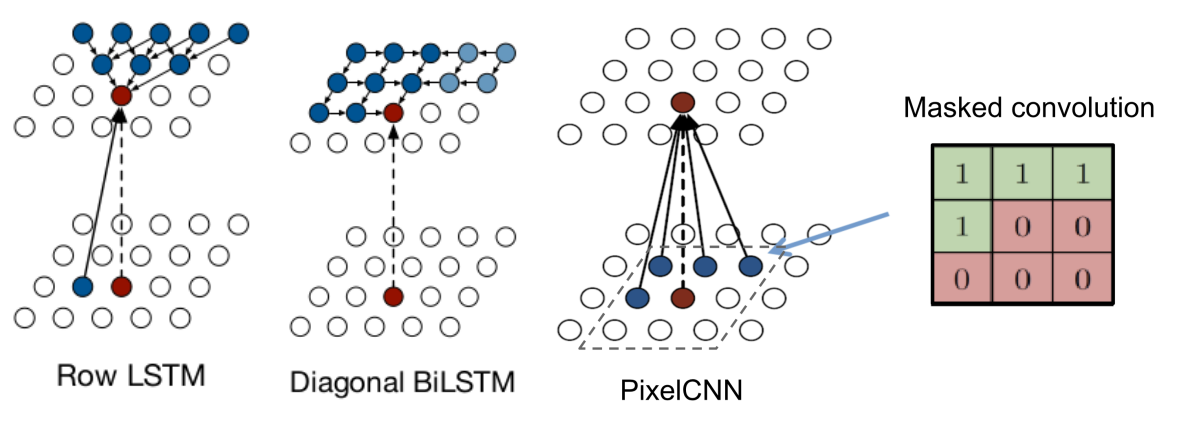
\includegraphics[width=\textwidth]{imgs/pixelrnn}
%	\caption{The process of Inverse Autoregressive Flows in Variational Autoencoder~\cite{kingma2016improved}.}
%	\label{fig:pixelrnn}
%\end{figure}

\subsection{Wavenet}
Wavenet~\cite{van2016wavenet} used the idea of Pixel CNN from~\cite{oord2016pixel} for raw audio generation. It used one-dimensional convolution Pixel CNN to generate raw audio. Wavenet has been proven to be the state-of-the-art model for text-to-speech model. Google Assistant in Android use wavenet to generate the audio of the assistant. 

Similar to Pixel CNN, the joint probability of an input audio is modelled by a stack of causal convolutional layers. Causal convolution has similar idea to masked convolution by shifting the output of a normal convolution by a few timesteps so it does not violate the autoregressive requirement. One of the problems with causal convolution is that it requires deep layers to capture long range dependency. The authors proposed to use dilated convolution where the convolution filter is applied over an area larger than its length. This is done by skipping input values with a certain step. 

\subsection{Glow}
Glow~\cite{kingma2018glow} extended and simplified the NICE and RealNVP model explained in Section~\ref{sec:realnvp} with three main extensions. First, the authors used activation normalization (act-norm) instead of batch normalization in RealNVP.  Act-norm performs a channel-wise normalization and is faster than batch normalization. Second, the authors used $1\times1$ convolution for the channel-wise permutation. NICE and RealNVP proposed a flow containing the equivalent of a permutation that reverses the ordering of the channels. This is changed with a $1\times1$ convolution so that the permutation can be learned.  Third, they extend RealNVP so that it can work faster by changing it into a multi-scale architecture. The authors splitted each step of the flow so it can be parallelized.

All of the additions mentioned before can be inverted and log-determinant of the Jacobian can be computed easily. Please refer to the paper for the details of the inversion and calculation of the Jacobian matrix. Glow has similar advantage as RealNVP that it can generate a high quality images. Moreover, the latent space learned by Glow is meaningful. This means that we can control the output of the generated image by tuning the latent space.


\section{Conclusion}
In this project, we have discussed how to transform a simple base distribution into a complex distribution by applying a series of invertible transformations called normalizing flows. We also discussed how normalizing flows can be applied to various representation learning regimes. Firstly, normalizing flows can be used for richer latent-posterior proposals for inference in the Variational Autoencoder. We discussed Planar and Radial Flows~\cite{rezende2015variational}, Inverse Autoregressive Flow~\cite{kingma2016improved}, and Sylvester Normalizing Flow~\cite{van2018sylvester} in this regime.  Secondly, normalizing flows can be used to estimate density when the exact likelihood is not known. We discussed NICE~\cite{dinh2014nice}, RealNVP~\cite{dinh2016density}, and Masked Autoregressive Flow~\cite{papamakarios2017masked} in this regime. We also discussed how normalizing flows can be implemented in deep probabilistic programming languages specifically Tensorflow Probability. Finally, we discussed several recent advances in normalizing flows used for image and audio generation.

In present day trends, applications of normalizing flows are being heavily used in methods involving variation inference. These are scalable methods which provide robust generative solutions. In contrast, auto-regressive methods suffer from slow sampling as the forward calculation of an autoregressive flow is not parallelizable. Density estimation methods ameliorate problems present in the mentioned methods, however their popularity remains constrained for historical reasons. Nevertheless, benchmark performance by models such as Glow seem to reverse this trend. From the PPL perspective, Tensorflow Probability provides the highest range of bijector families, thus making it the ideal choice for flow-based implementations. 

%
% ---- Bibliography ----
%
% BibTeX users should specify bibliography style 'splncs04'.
% References will then be sorted and formatted in the correct style.
%
% \bibliographystyle{splncs04}
% \bibliography{mybibliography}
%
\bibliographystyle{splncs04}
\bibliography{ref} 




\appendix


\section{Contribution}
\subsection*{Abdul Fatir Ansari}
\begin{enumerate}
	\item Introduction \& Background (Autoencoder \& Variational Autoencoder)
	\item Applications
	\begin{itemize}
		\item Variational Inference using Normalizing Flows (basics)
		\item Planar and Radial Flow
		\item Sylvester Normalizing Flow
		\item Masked Autoregressive Flow
	\end{itemize}
	\item Normalizing flows in PPLs
	\item Appendix: Implementation of planar flow with experiments on two complex densities
	\item Problem Set 1
	\item Code examples
\end{enumerate}

\subsection*{Devamanyu Hazarika}
\begin{enumerate}
	\item Applications
	\begin{itemize}
		\item Normalizing Flows for Density Estimation 
		\item Non-linear Independent Components Estimation
		\item Real-valued Non-Volume Preserving
	\end{itemize}
	\item Conclusion
    \item Appendix: Jacobian for affine transformation and discussion
    \item Problem Set 2: Question 2
\end{enumerate}


\subsection*{Remmy A. M. Zen}
\begin{enumerate}
	\item Applications
	\begin{itemize}
		\item Inverse Autogregressive Flow
	\end{itemize}
	\item Normalizing flows in PPLs
	\item Recent advances
	\item Conclusion
	\item Problem Set 2: Question 1
\end{enumerate}

\section{Appendix (Abdul Fatir Ansari)}

\subsection{Planar and Radial Flow Derivations}

\paragraph{Planar Flow} Differentiating Eq. (\ref{eq:planarfn}), the Jacobian is given by
\begin{align*}
\frac{\partial f(\mathbf{z})}{\partial \mathbf{z}} = \mathbf{I} + \mathbf{u}h'(\mathbf{w}^\top\mathbf{z} + b)\mathbf{w}^\top
\end{align*}

Now, using the matrix determinant lemma
\begin{align}
\det\frac{\partial f(\mathbf{z})}{\partial \mathbf{z}} &= (1 + h'(\mathbf{w}^\top\mathbf{z} + b)\mathbf{w}^\top\mathbf{I}^{-1}\mathbf{u})\det(\mathbf{I})\\
&=(1 + h'(\mathbf{w}^\top\mathbf{z} + b)\mathbf{w}^\top\mathbf{u})\label{eq:planar-det}
\end{align}
\paragraph{Radial Flow} Differentiating Eq. (\ref{eq:radialfn}), the Jacobian is given by
\begin{align*}
\frac{\partial f(\mathbf{z})}{\partial \mathbf{z}} &= \mathbf{I} + \beta\left((\mathbf{z}-\mathbf{z}_0)h'(\alpha,r)\frac{\partial r}{\partial \mathbf{z}} + h(\alpha,r)\mathbf{I}\right)\\
&=(1+\beta h(\alpha,r))\mathbf{I} + \beta h'(\alpha,r)(\mathbf{z}-\mathbf{z}_0)\frac{(\mathbf{z}-\mathbf{z}_0)^\top}{||\mathbf{z}-\mathbf{z}_0||}
\end{align*}

Let $\gamma = (1+\beta h(\alpha,r))$. Using the matrix determinant lemma
\begin{align}
\det\frac{\partial f(\mathbf{z})}{\partial \mathbf{z}} &= \left(1 + \beta h'(\alpha,r)\frac{(\mathbf{z}-\mathbf{z}_0)^\top}{||\mathbf{z}-\mathbf{z}_0||}\frac{\mathbf{I}}{\gamma}(\mathbf{z}-\mathbf{z}_0)\right)\det(\gamma\mathbf{I})\\
&=\left(\frac{1 + \beta h(\alpha,r) + \beta h'(\alpha,r)||\mathbf{z}-\mathbf{z}_0||}{(1+\beta h(\alpha,r))}\right)(1+\beta h(\alpha,r))^d\\
&=\left(1 + \beta h(\alpha,r) + \beta h'(\alpha,r)r\right)(1+\beta h(\alpha,r))^{d-1}\label{eq:radial-det}
\end{align}

\subsection{Code for PReLU}
\begin{code}
	\inputminted[linenos=true,frame=lines,framesep=2mm]{python}{prelu.py}
	\captionof{listing}{Parametrized ReLU Bijector}
\end{code}

\subsection{Reproducing Results from Rezende and Mohamed~\cite{rezende2015variational}}
Reproducibility is an important concern in deep learning, especially because the models are trained stochastically in environments that can be very different from each other.  With this is mind, and a lack of official implementation from the authors, I implemented planar flows and conducted a few experiments presented in the paper. 

The experiment seeks to approximate two complex 2D densities using planar flows. The unnormalized density functions are given by $p(\mathbf{z}) \propto e^{-U_i(\mathbf{z})}$ where the two energy functions $U_1$ and $U_2$ are
\begin{align}
U_1(\mathbf{z}) &= \frac{1}{2}\left(\frac{\|\mathbf{z}\| - 4}{0.4}\right)^2 - \log \left(e^{-\frac{1}{2}\left[\frac{z_1-2}{0.8}\right]^2} + e^{-\frac{1}{2}\left[\frac{z_1+2}{0.8}\right]^2} \right)\\
U_2(\mathbf{z}) &= \frac{1}{2}\left[\frac{z_2 - \sin\left(\frac{2\pi z_1}{4}\right)}{0.4}\right]^2
\end{align}

\begin{figure}
	\centering
	\subfloat[Density 1]{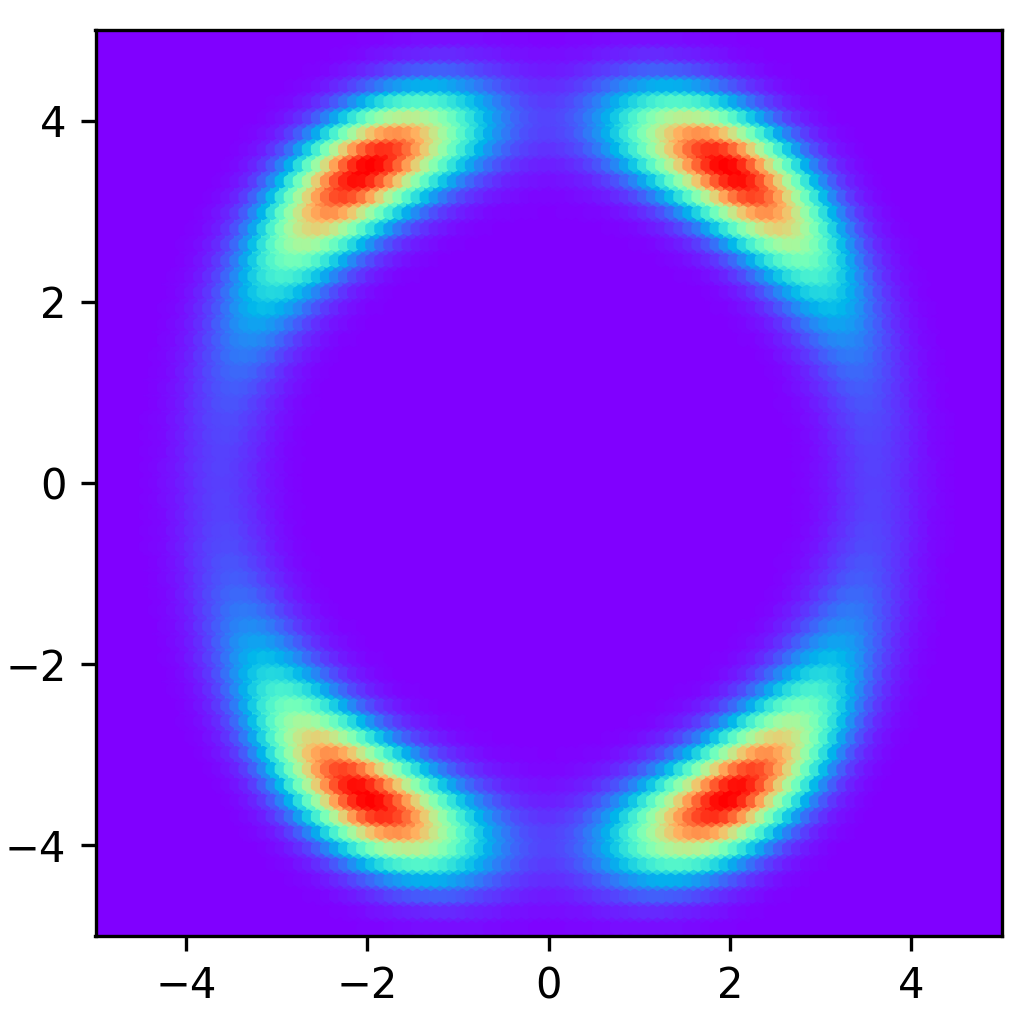
\includegraphics[width=0.3\textwidth]{example1-density}}
	\subfloat[Samples from 1]{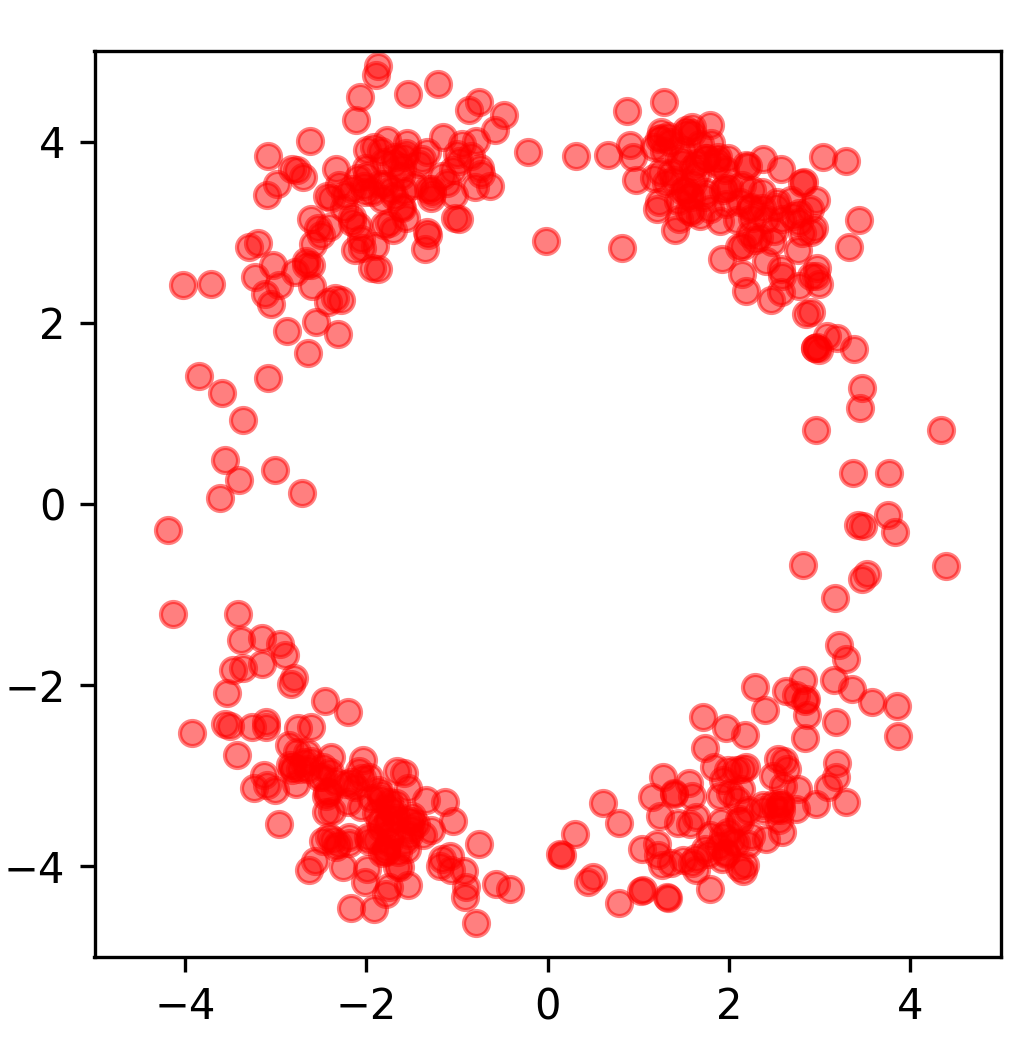
\includegraphics[width=0.3\textwidth]{example1-samples}}\\
	\subfloat[Density 2]{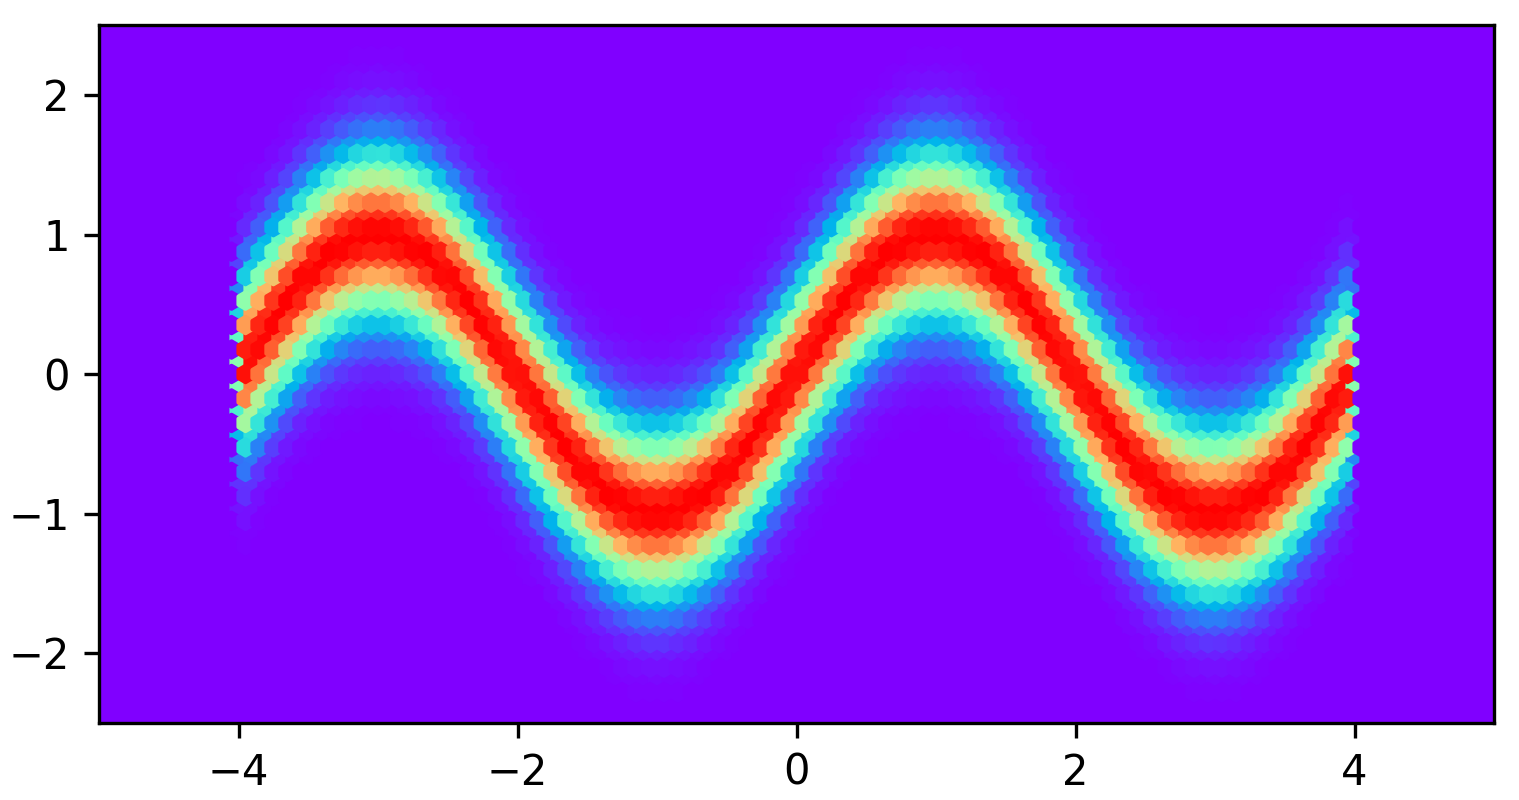
\includegraphics[width=0.3\textwidth]{example2-density}}
	\subfloat[Samples from 2]{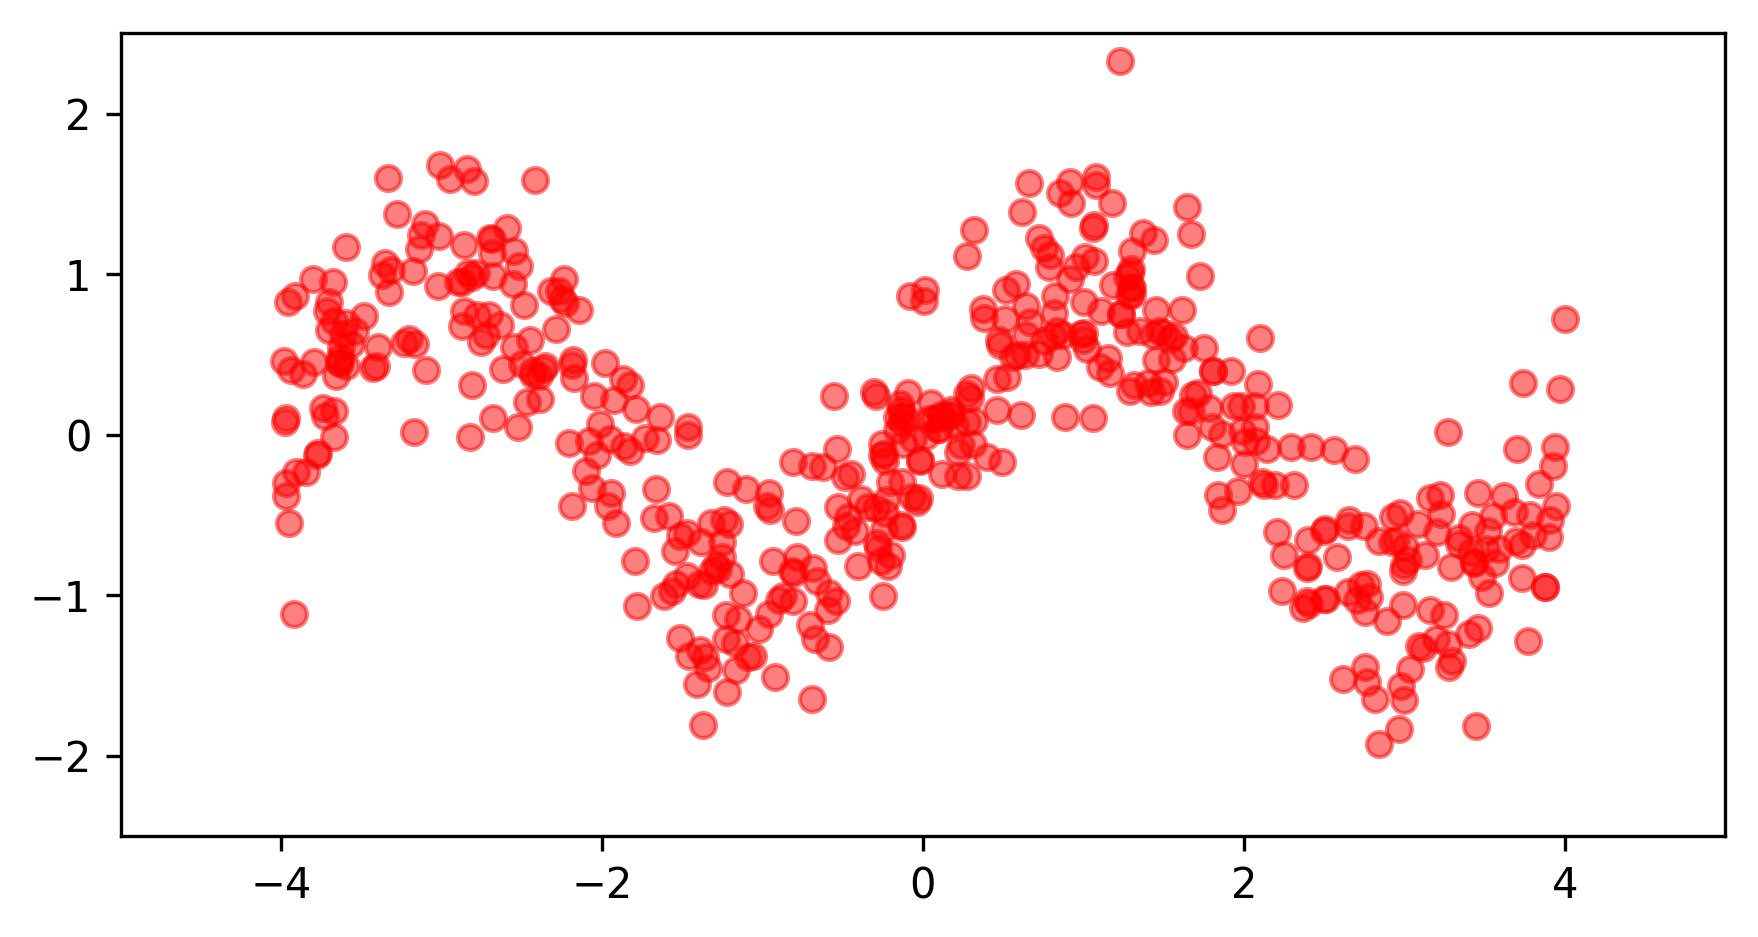
\includegraphics[width=0.3\textwidth]{example2-samples}}\\
	\caption{Two probability densities and samples from each density obtained using Metropolis-Hastings}
	\label{fig:densities}
\end{figure}

\begin{figure}
	\centering
	\subfloat[K = 2]{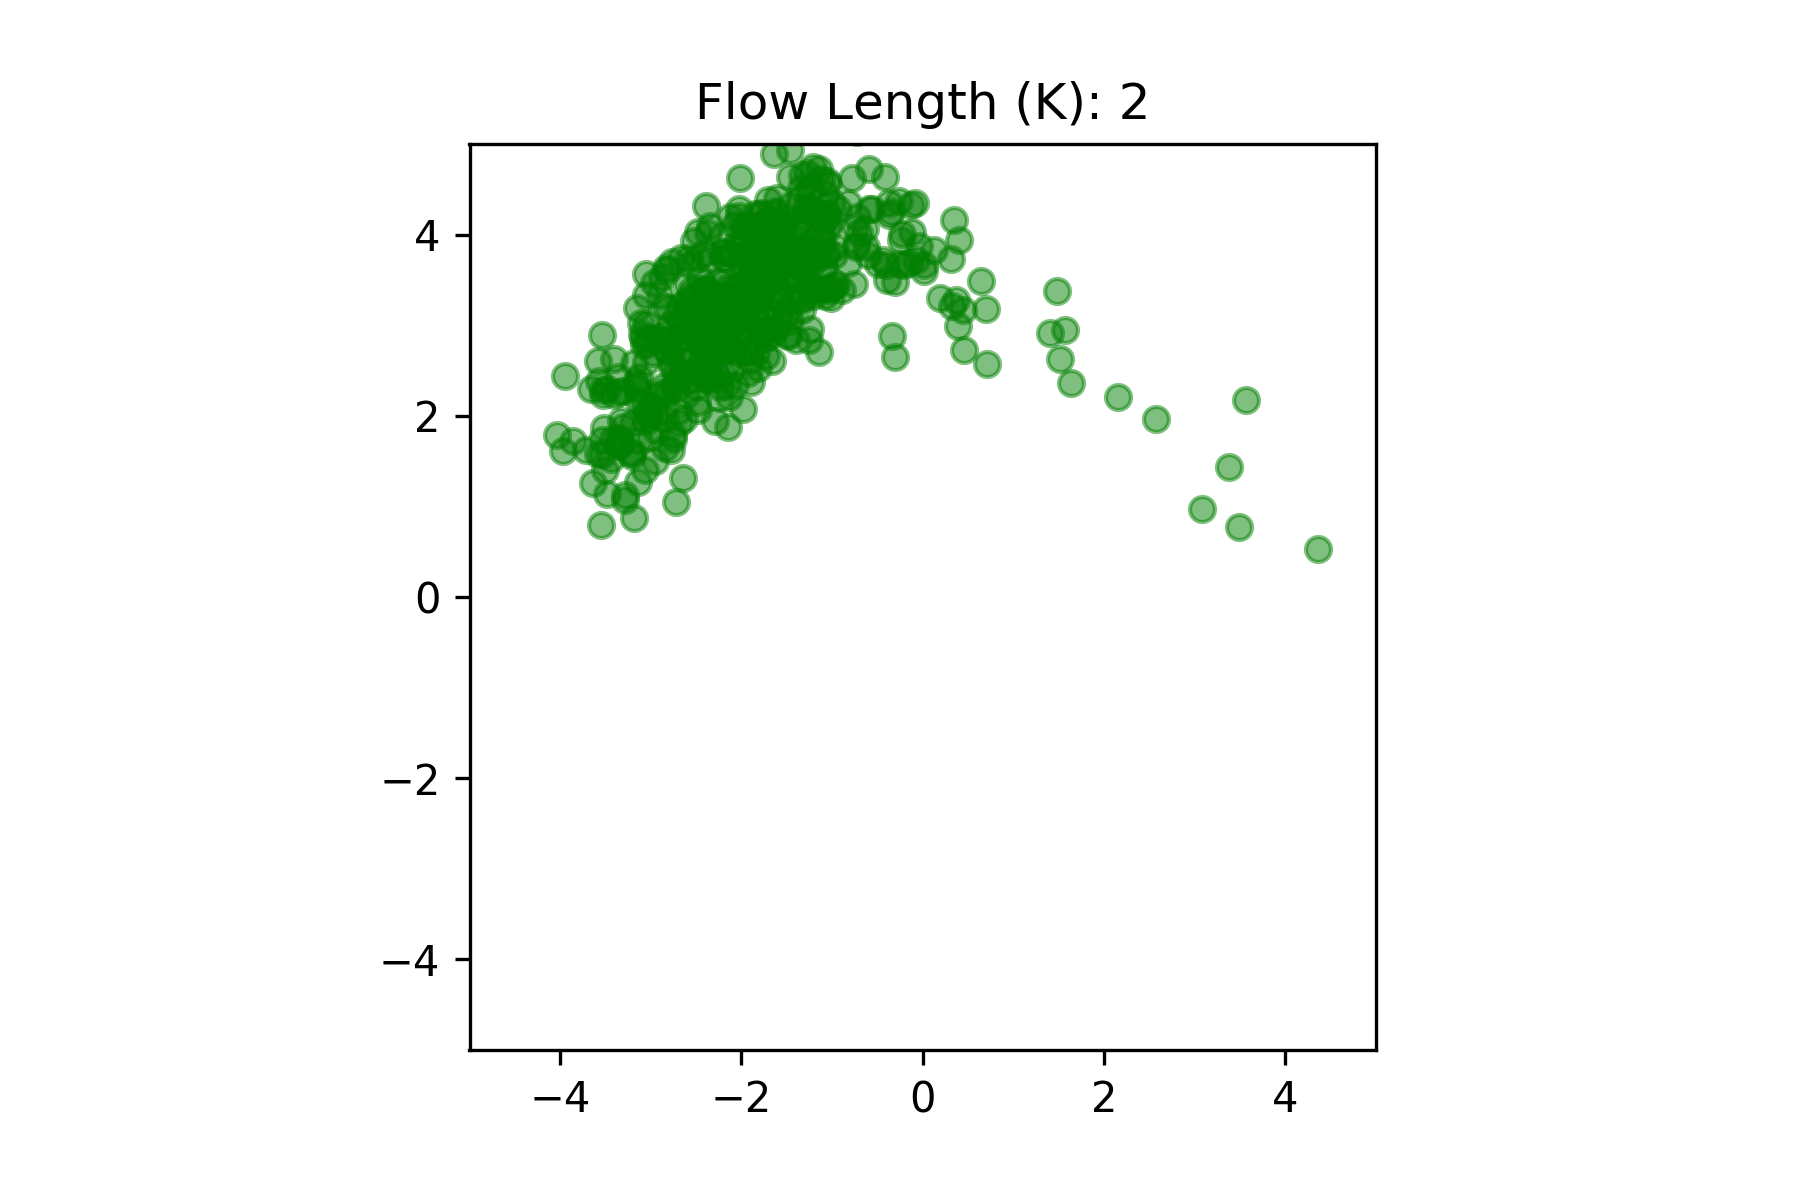
\includegraphics[width=0.3\textwidth]{example1-k2}}
	\subfloat[K = 4]{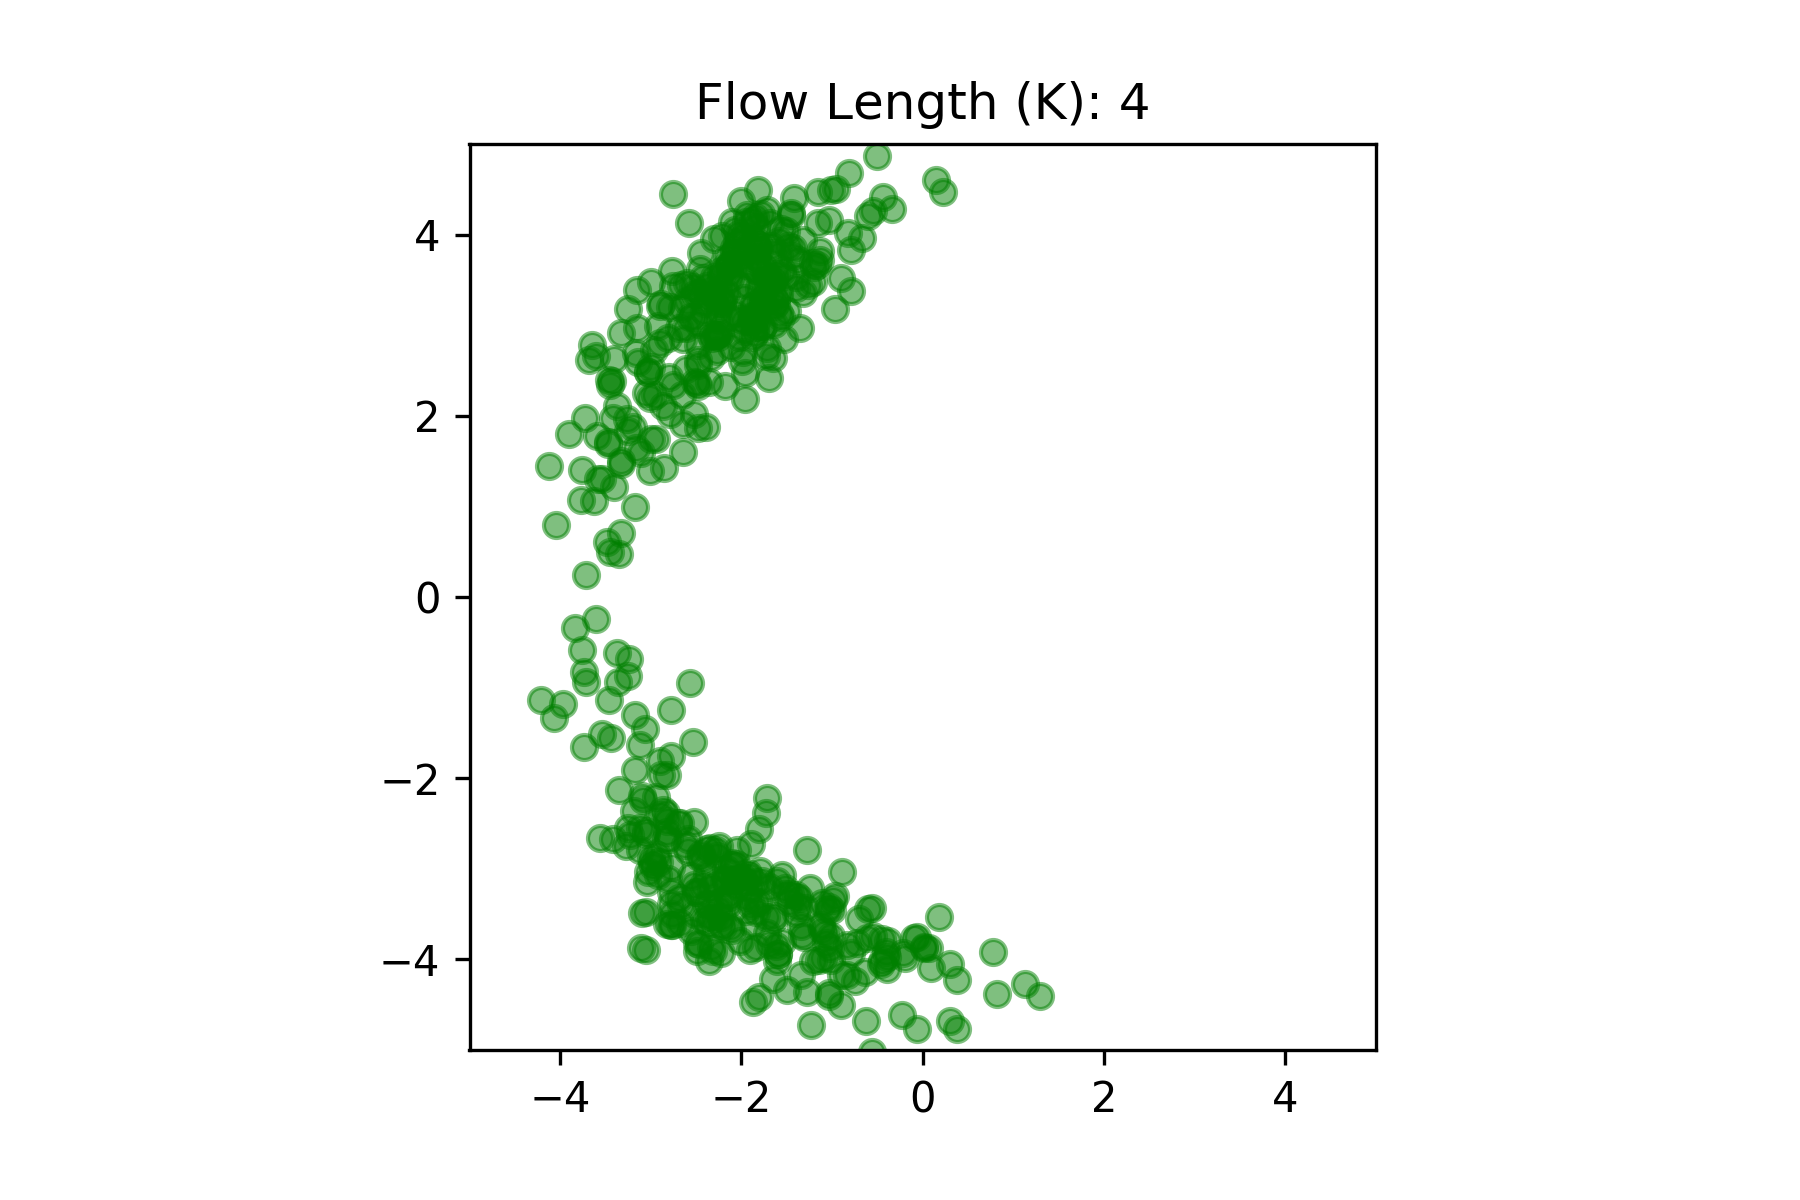
\includegraphics[width=0.3\textwidth]{example1-k4}}\\
	\subfloat[K = 8]{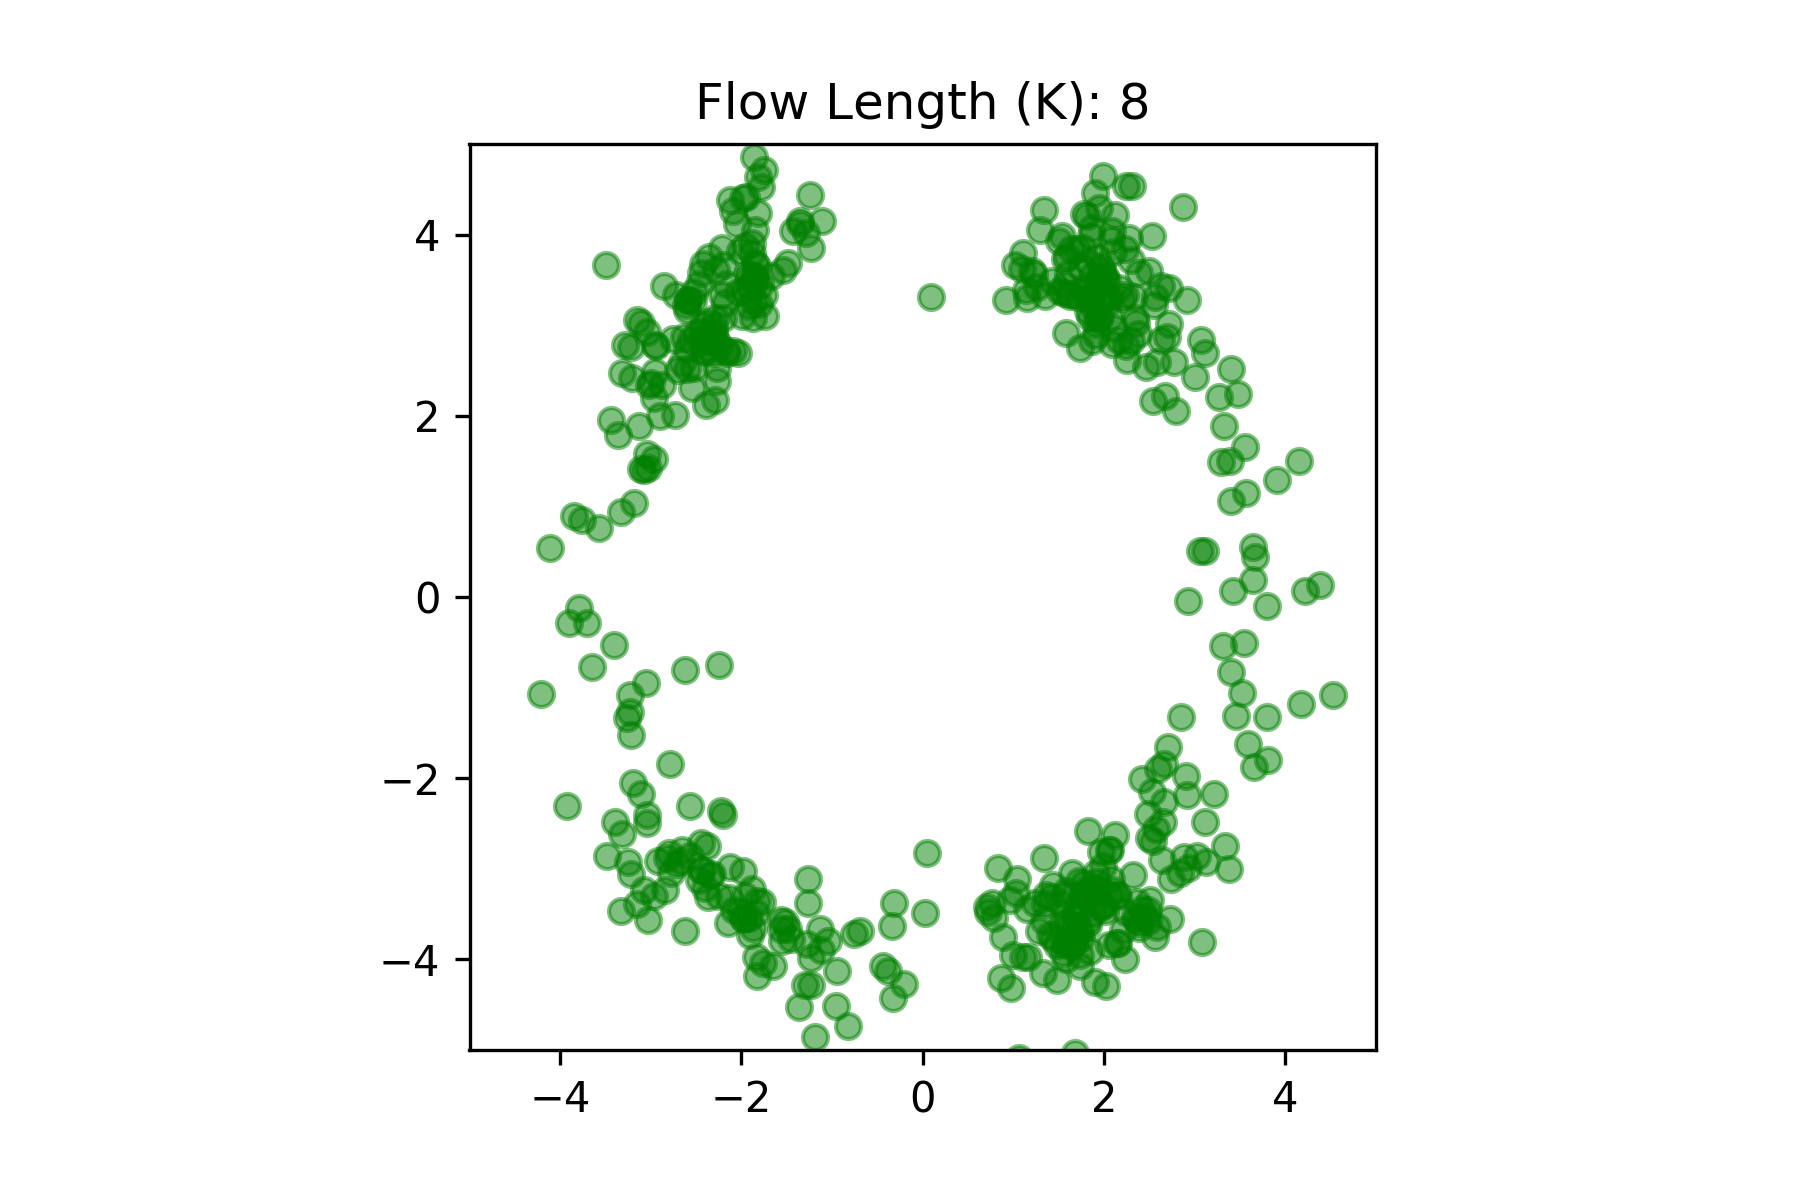
\includegraphics[width=0.3\textwidth]{example1-k8}}
	\subfloat[K = 16]{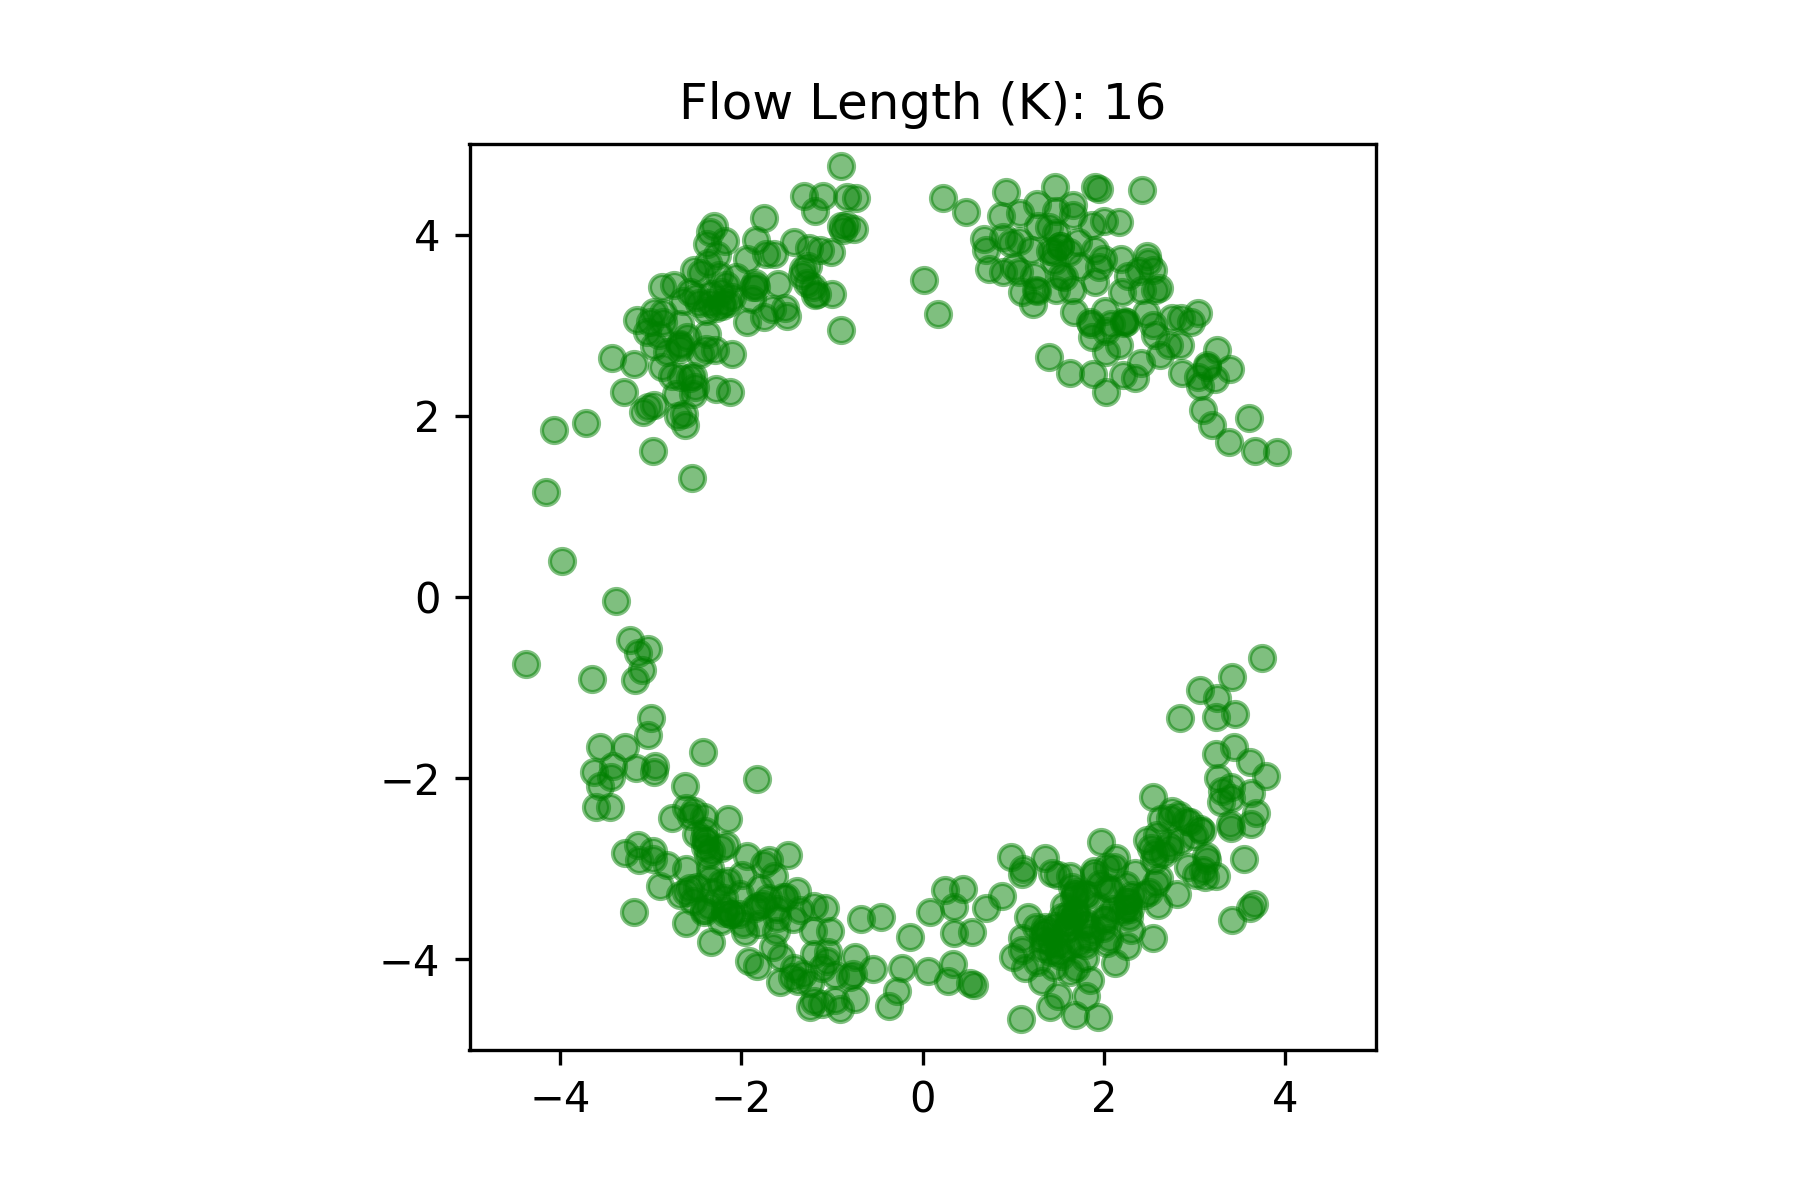
\includegraphics[width=0.3\textwidth]{example1-k16}}\\
	\caption{500 samples from Planar Flows with different flow lengths after 10000 training steps for density 1}
	\label{fig:density1}
\end{figure}

\begin{figure}
	\centering
	\subfloat[K = 2]{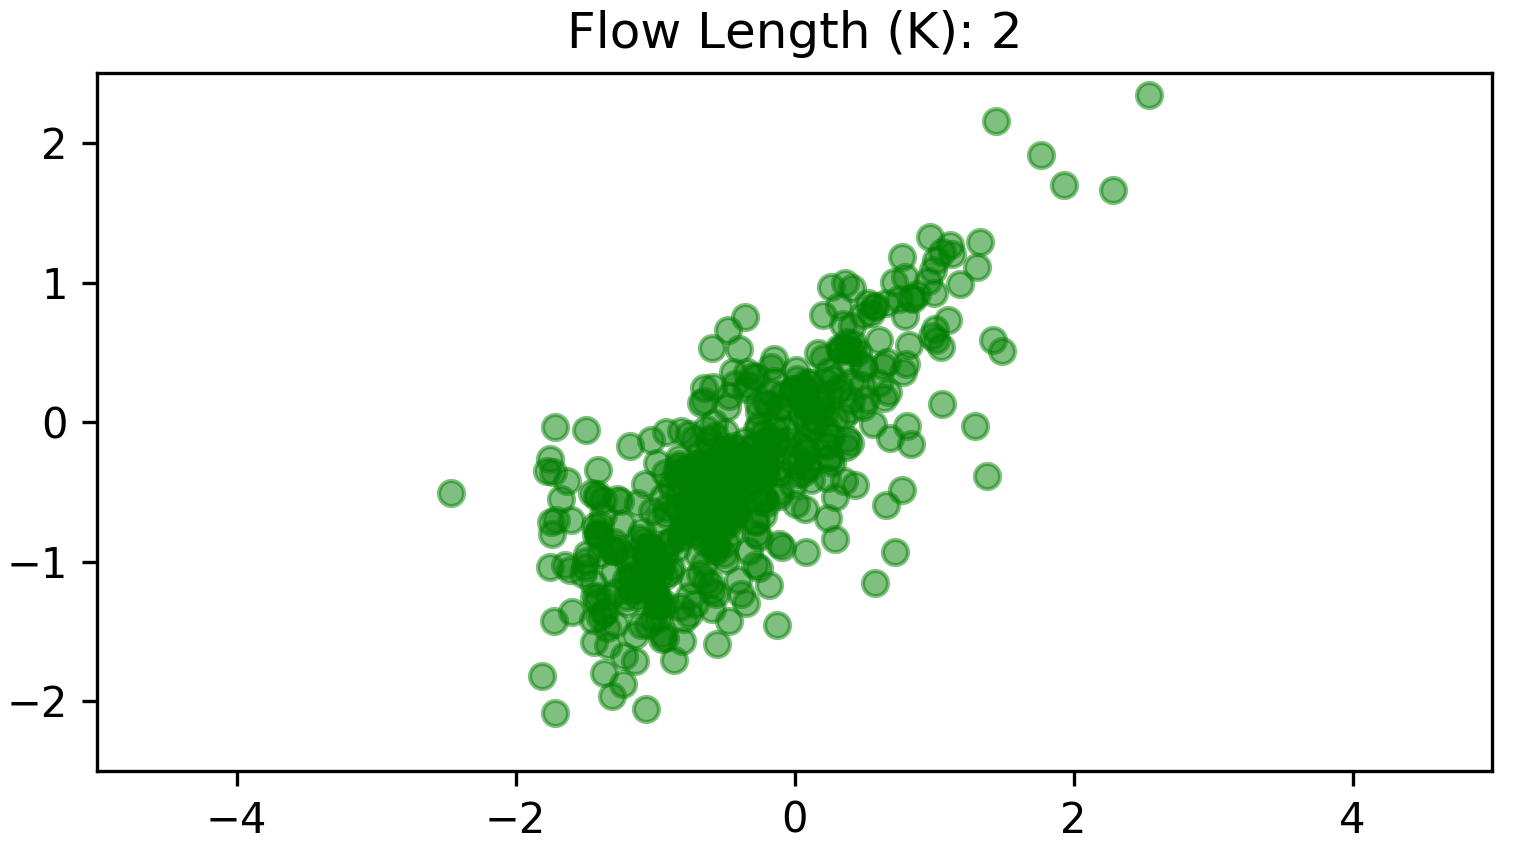
\includegraphics[width=0.3\textwidth]{example2-k2}}
	\subfloat[K = 4]{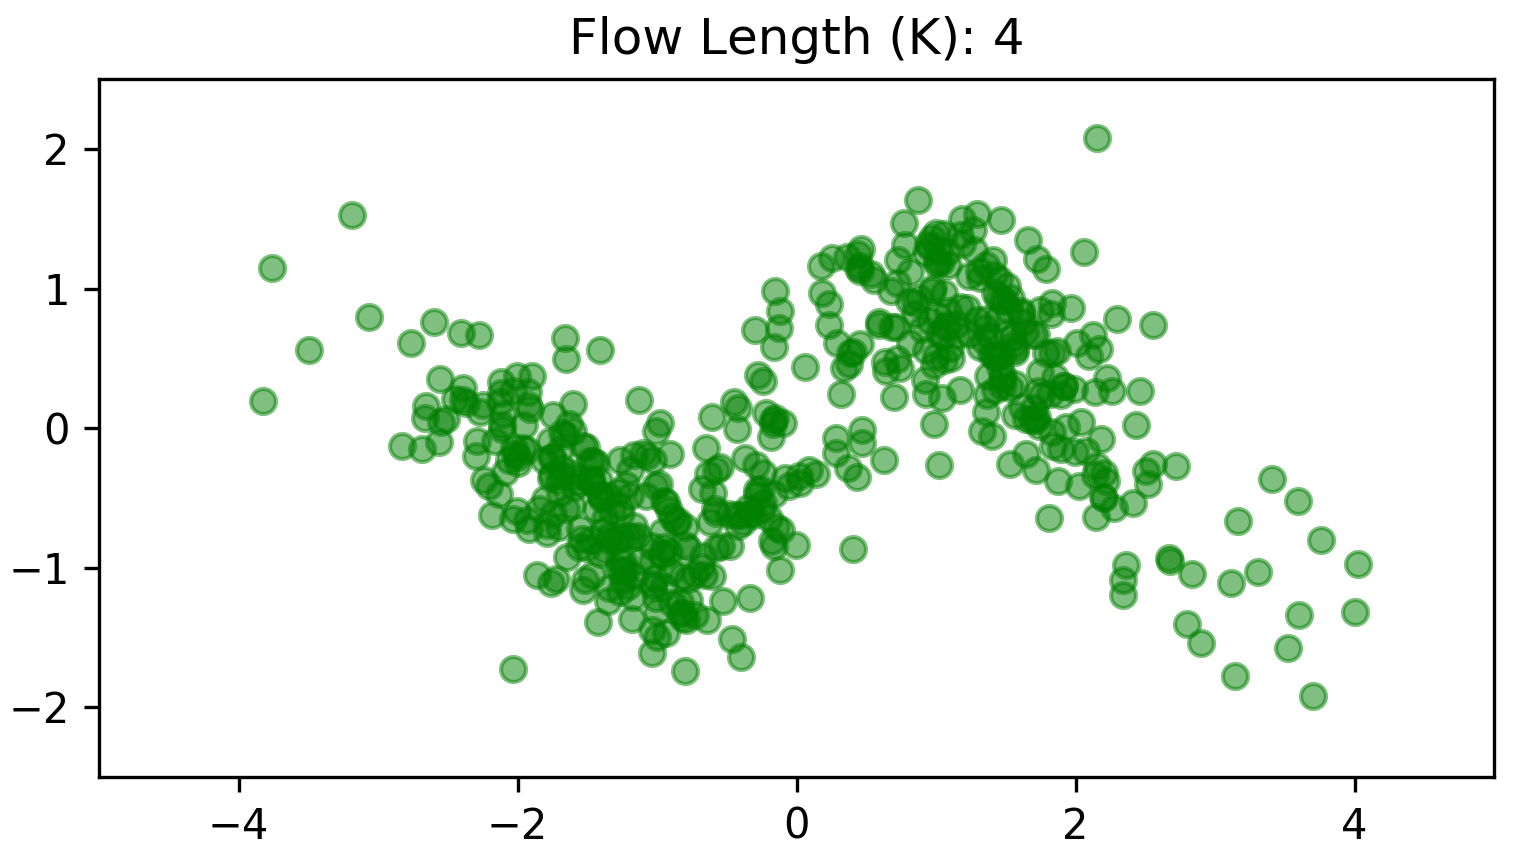
\includegraphics[width=0.3\textwidth]{example2-k4}}\\
	\subfloat[K = 8]{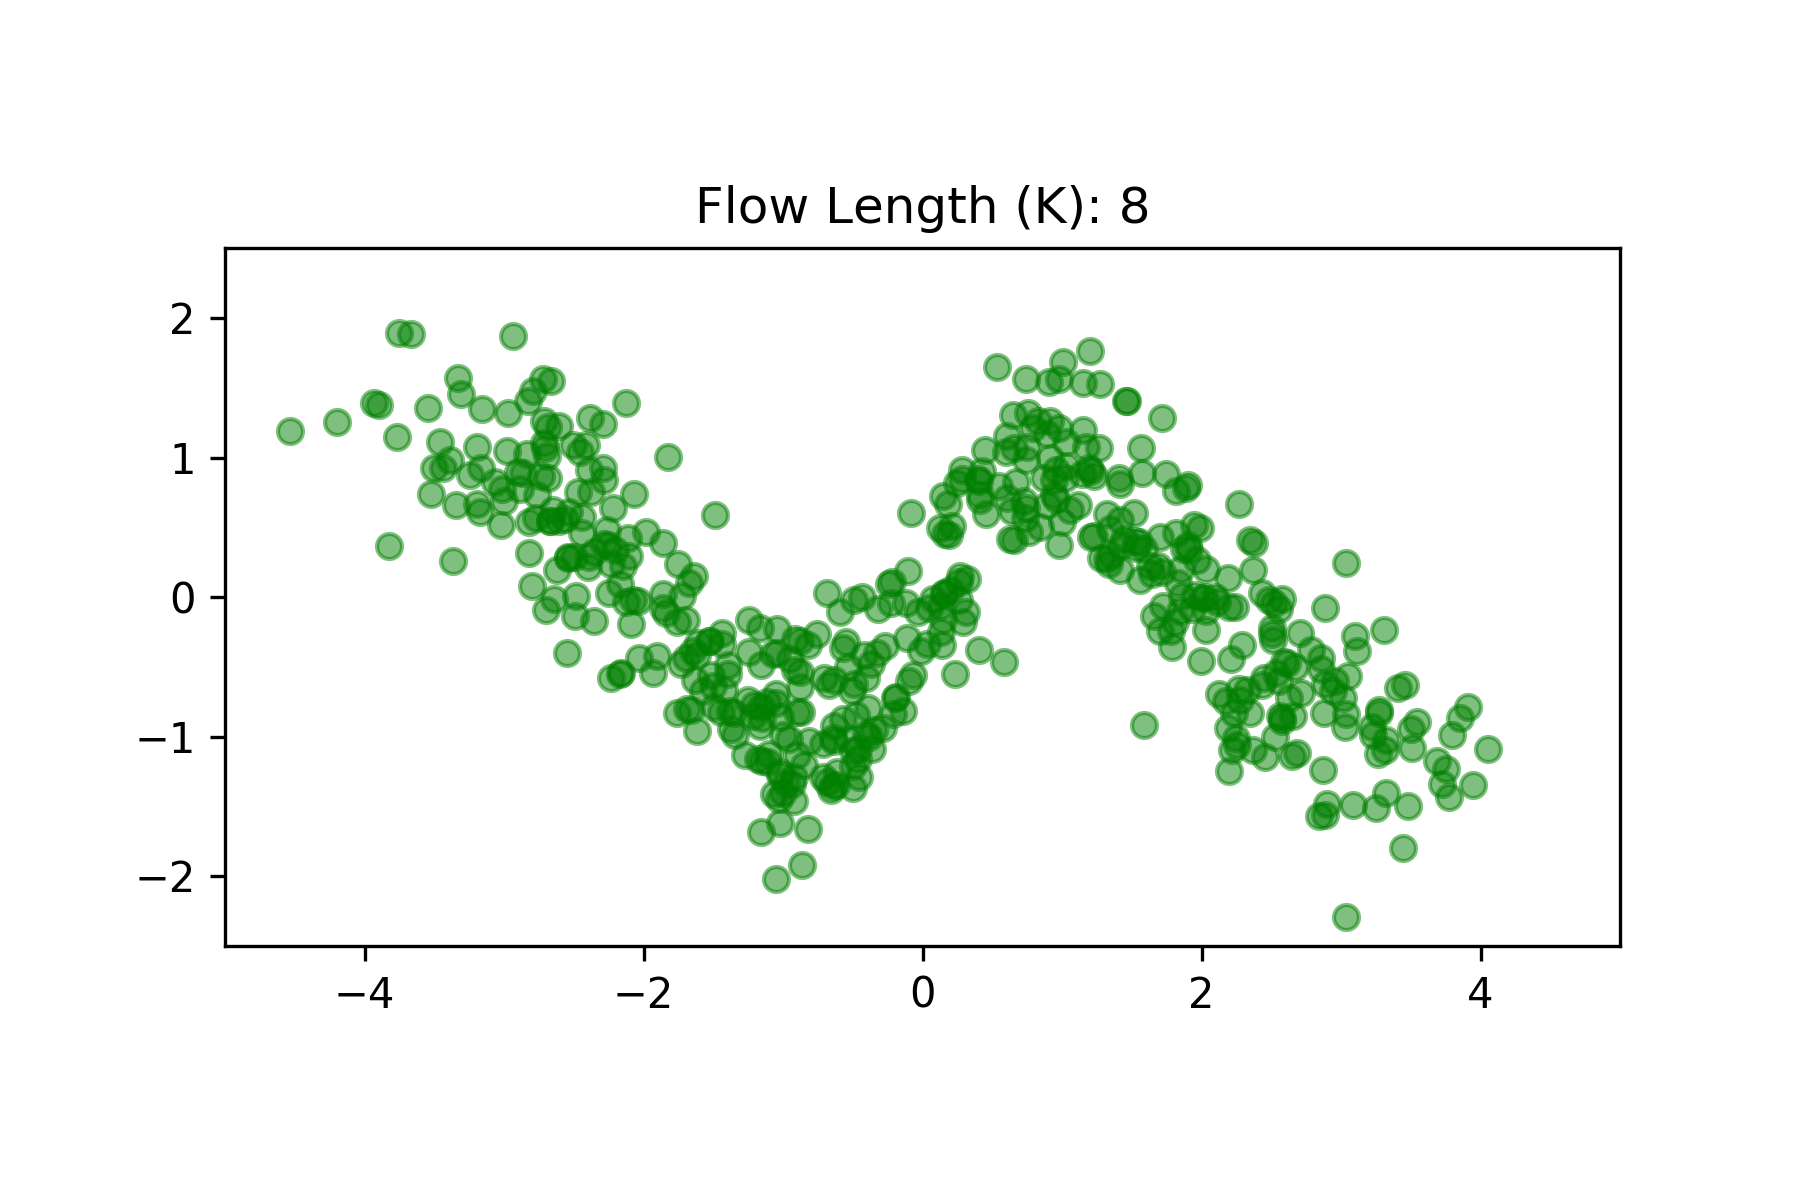
\includegraphics[width=0.3\textwidth]{example2-k8}}
	\subfloat[K = 16]{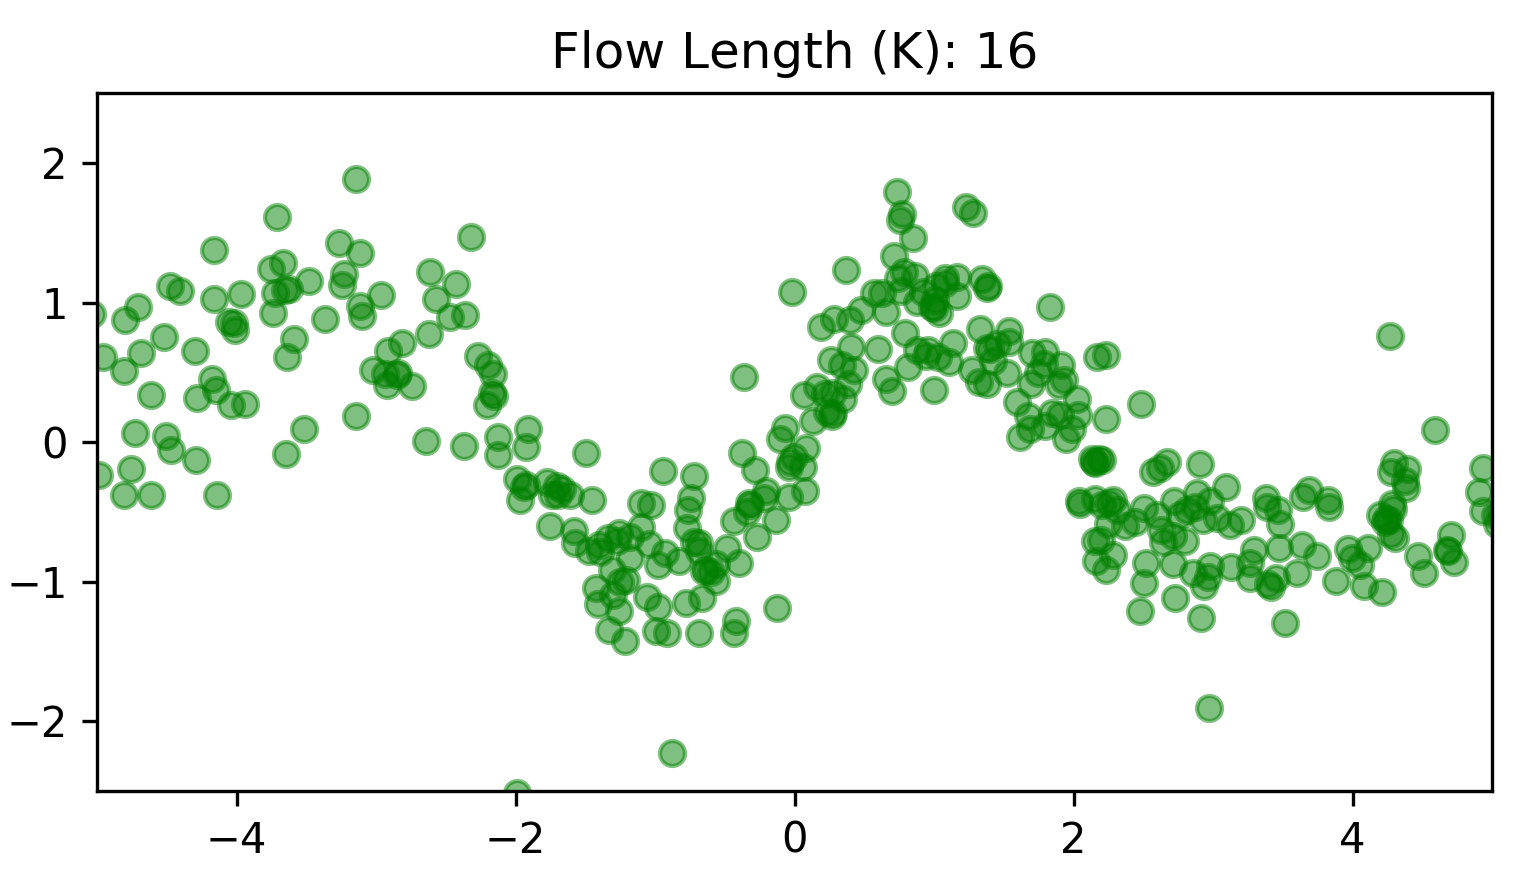
\includegraphics[width=0.3\textwidth]{example2-k16}}\\
	\caption{500 samples from Planar Flows with different flow lengths after 5000 training steps for density 2}
	\label{fig:density2}
\end{figure}

Fig. \ref{fig:densities} shows the two densities along with a scatter plot of 500 samples from each density obtained using Metropolis-Hastings (MH) algorithm. The MH algorithm was implemented in \texttt{numpy} using the normal distribution with identity covariance matrix as the proposal distribution. A part of the code that implements the MH algorithm is given in Snippet \ref{code:mh}. See \texttt{Metropolis-Hastings.ipynb} for complete code.

Planar Flow was implemented in Tensorflow and the code satisfies the invertibility conditions mentioned in the appendix of~\cite{rezende2015variational}. Tensorflow Probability (TFP) was not used because it requires implementation of the \texttt{\_inverse} function which is not available for the function used in planar flows although they are invertible. Flow lengths ($K$) from the set $\{2, 4, 8, 16\}$ were tested and trained using the Adam optimizer. A part of the code that implements planar flow is given in Snippet \ref{code:planar}. See \texttt{PlanarFlow-Example1.ipynb} and \texttt{PlanarFlow-Example2.ipynb} for complete code. Note that constant terms were dropped during the computation of the KL-divergence which may lead to negative KL values.

Figs. \ref{fig:density1} and \ref{fig:density2} show samples from planar flows of different lengths for density 1 and density 2 respectively at the end of training. It is clear from the results that as flow length increases, the model is able to better approximate the true density. Another interesting aspect encountered during the course of experiments was that the training becomes unstable as length of flow $K$ increases, especially for density 2. 

\begin{code}
	\inputminted[linenos=true,frame=lines,framesep=2mm]{python}{metropolis.py}
	\captionof{listing}{Metropolis-Hastings}
	\label{code:mh}
\end{code}
\begin{code}
	\inputminted[linenos=true,frame=lines,framesep=2mm]{python}{planar.py}
	\captionof{listing}{Planar Flow}
	\label{code:planar}
\end{code}

\section{Appendix (Devamanyu Hazarika)}

First, let us derive the Jacobian for the affine coupling law defined in RealNVP:

\begin{align*}
\frac{\partial \mathbf{y}}{\partial \mathbf{x^T}} &= \begin{bmatrix}
\frac{\partial y_{1:d}}{\partial x_{1:d}} & \frac{\partial y_{1:d}}{\partial x_{d+1:D}} \\
\frac{\partial y_{d+1:D}}{\partial x_{1:d}} & \frac{\partial y_{d+1:D}}{\partial x_{d+1:D}} 
\end{bmatrix}\\
&= \begin{bmatrix}
I_{d} & 0 \\
\frac{\partial y_{d+1:D}}{\partial x_{1:d}} & \frac{\partial \left(x_{d+1:D} \odot \exp\left((s(x_{1:d})\right)) + t(x_{1:d})\right)}{\partial x_{d+1:D}} 
\end{bmatrix}\\
&= \begin{bmatrix}
I_{d} & 0 \\
\frac{\partial y_{d+1:D}}{\partial x_{1:d}} & diag\left(\,\exp[s(x_{1:d})]\right)
\end{bmatrix}
\end{align*}

Thus, the corresponding log determinant is:
\begin{align*}
\log\left( \left|\det(\frac{\partial \mathbf{y}}{\partial \mathbf{x^T}})\right|\right) &= \sum_{i=1}^{d}{\log(\exp(s(x_i)))}
\end{align*}
which can be calculated in $O(d)$ time.

\paragraph{Discussion:}
In their results, RealNVP doesn not surpass the state-of-the-art models. But it contains certain advantages over other proposed approaches. Firstly, compared to variational methods, density estimation methods provide tractable and exact log-lkelihood evaluation. This makes the model much more flexible. Secondly, there is no explicit likelihood function required with terms comprising reconstruction loss. This allows the generated images to be sharper compared to other approaches such as variational autoencoders. Thirdly, unlike auto-regressive flows, the sampling scheme can be parallelized and thus modern hardware can be used to fasten the process.

When considering the discussed density estimation methods with other models such as VAEs and GANs, one key difference arises in the size of the latent space. RealNVP and similar techniques are able to find meaningful latent dimensions in a space with similar dimensions as the input. In contrast, other methods try to find meaningful latent states which are low dimensional. The former approach presents better expressibility and is thus desirable. 

\end{document}
